\documentclass[]{article}

\usepackage{graphicx}
\graphicspath{ {Images/} }
\usepackage{titlesec}
\usepackage[top=1in, bottom=0.8in, left=1.2in, right=1.2in]{geometry}

\titleformat{\section}
  {\normalfont\Large\bfseries}{\thesection}{1em}{}[{\titlerule[0.8pt]}]

\begin{document}

\section*{Python STEM Initiative: Installing Anaconda}
Hello there! \\

Welcome to the 2017 Python STEM Initiative. This document will help you download the tools you need to get started with Python. We will be using the Python distribution knows as Anaconda. Anaconda comes with a vast amount of libraries, Jupyter Notebooks with iPython, and has nice cross-platform support. Anaconda can be obtained for free from www.continuum.io. We've left detailed directions on installing and getting started with Anaconda below. Also below you'll find our contact information. We are always available via email if you have questions. If you do send us an email, please include the phrase "Python STEM Initiative" in the subject line.

Cheers, \\

Joel Anderson \\
joel.s.anderson@stonybrook.edu\\ \\

Bryan Sundahl \\
bryan.sundahl@stonybrook.edu

\paragraph{}
The instructions from this point on will be for Mac users, since we guess that will cover most students' needs. Windows and Linux installations are nearly identical.
\paragraph{}
First, open your web browser (Edge, Chrome, Firefox, Safari, etc.) and in the url bar type continuum.io
\paragraph{}
\begin{centering}
    \centerline{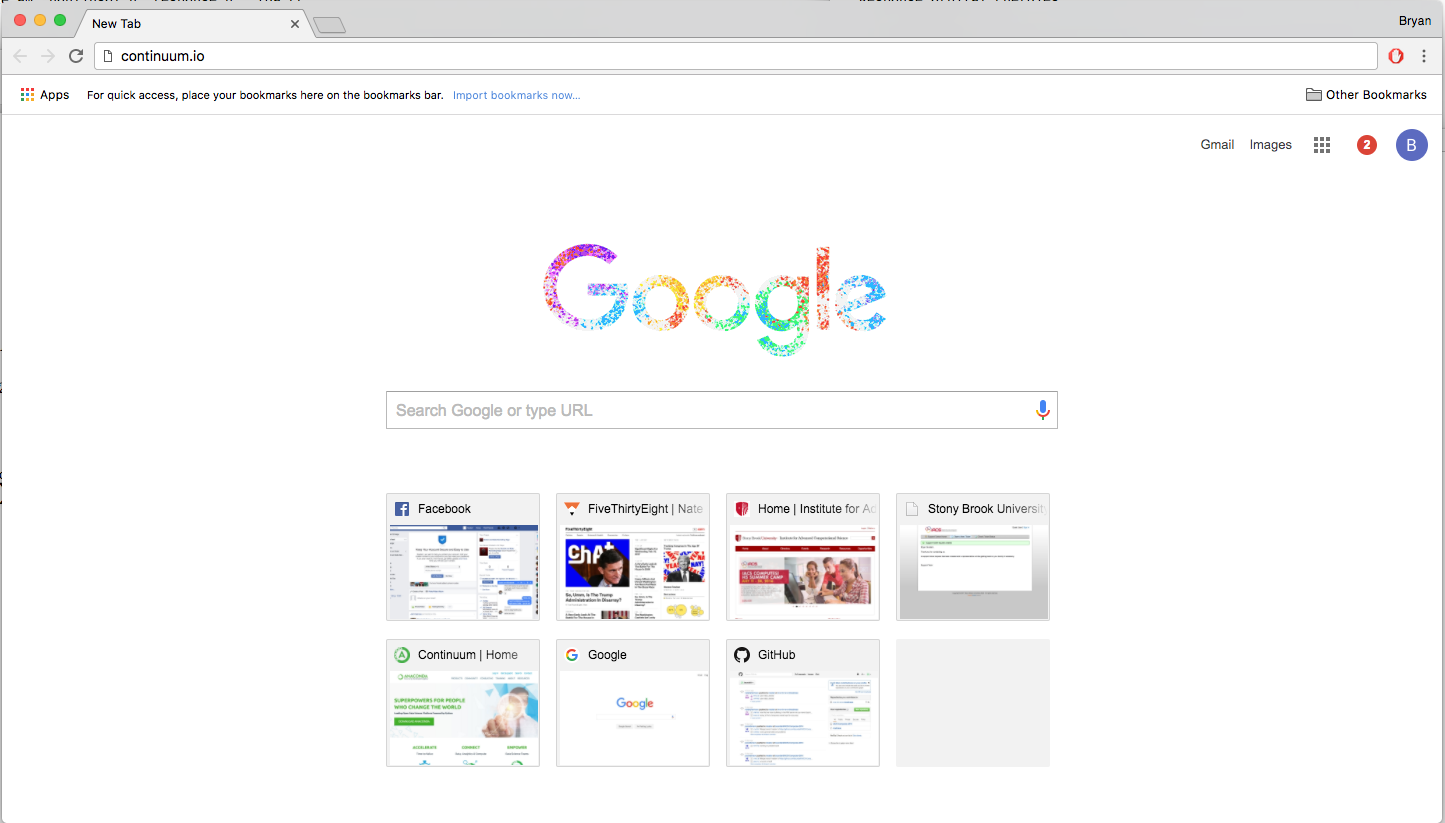
\includegraphics[scale=0.35]{Screenshot_1.png}}
\end{centering}

\paragraph{}
On the continuum.io website, click on the large green Download Anaconda button
\paragraph{}
\begin{centering}
    \centerline{
\includegraphics[scale=0.35]{Screenshot_2.png}}
\end{centering}

\paragraph{}
If you scroll down, you should see an image that looks like the one below (You may need to first choose the macOS icon at the top of the screen). Make sure you're looking at the one that says "Anaconda for macOS." Click on the macOS 64-Bit Graphical Installer on for Python 3.6.
\paragraph{}
\begin{centering}
    \centerline{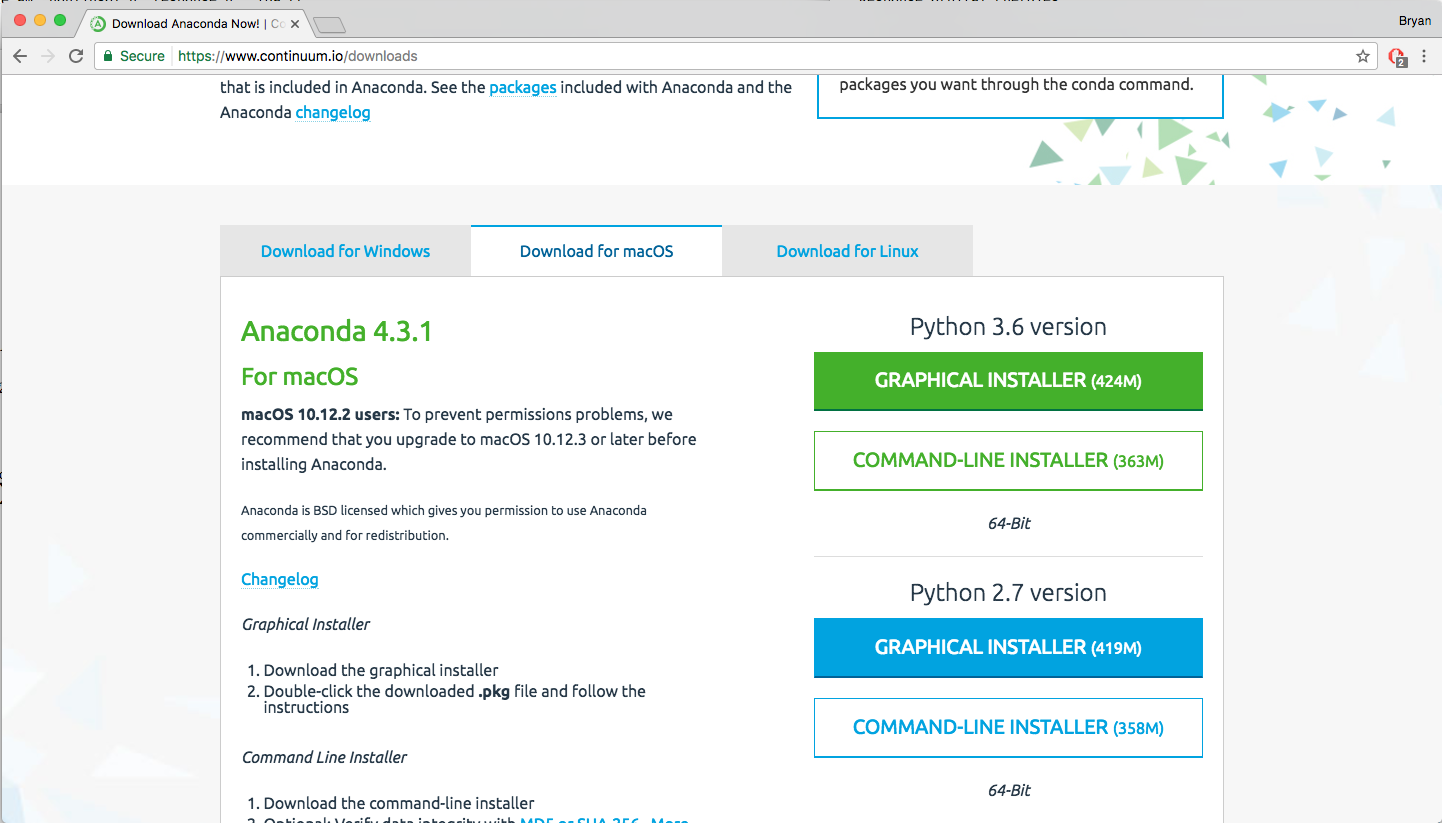
\includegraphics[scale=0.35]{Screenshot_3.png}}
\end{centering}

\paragraph{}
Wait for the file to download, then find the downloaded file and click on it to execute. If you're using Chrome, this can simply be accomplished by clicking the file in the tray at the bottom of the brower.

Note: If you are having issues getting the installation executable to download on Windows, try downloading the .zip version from the website. Please verify that the .zip you are downloading is for Anaconda3 (64 bit version if you have a 64 bit operating system - if you don't know what I'm talking about, pick the file with 64.zip on the end of it.)

\paragraph{}
\begin{centering}
    \centerline{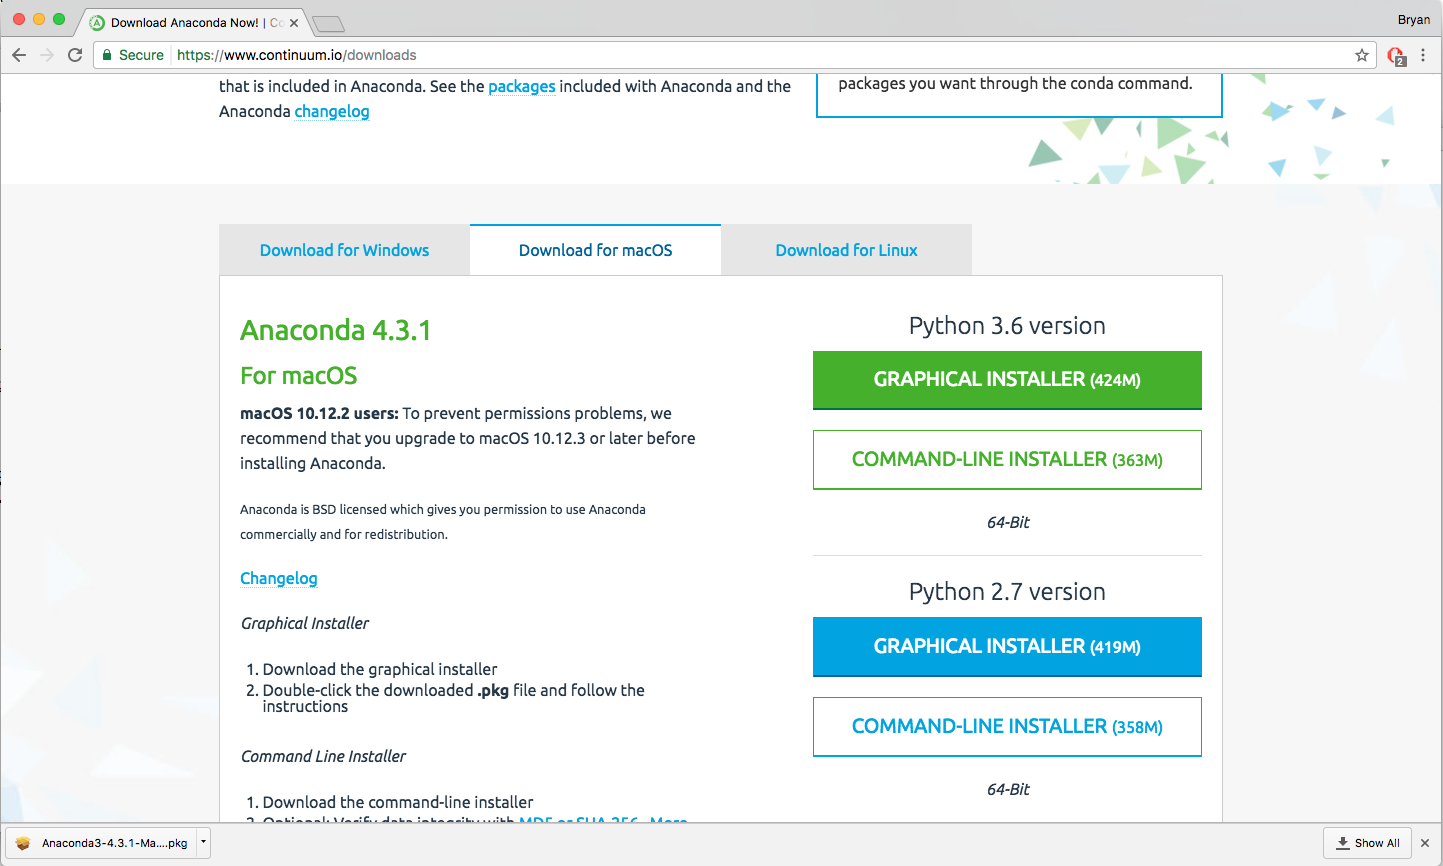
\includegraphics[scale=0.35]{Screenshot_4.png}}
\end{centering}

\paragraph{}
You should see a window pop up like the one below. Click "Continue" three times.
\paragraph{}
\begin{centering}
    \centerline{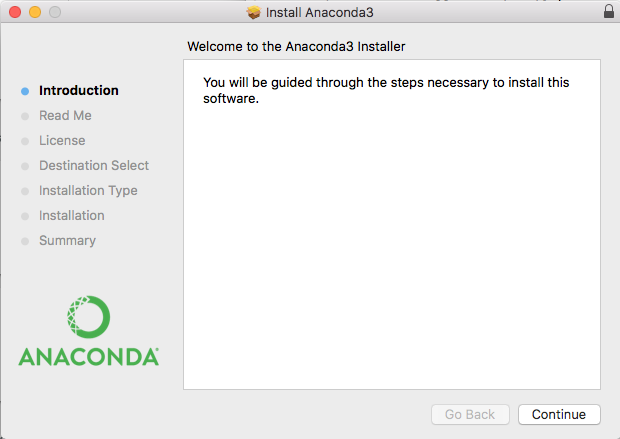
\includegraphics[scale=0.7]{Screenshot_5.png}}
\end{centering}

\paragraph{}
Then click I Agree.
\paragraph{}
\begin{centering}
    \centerline{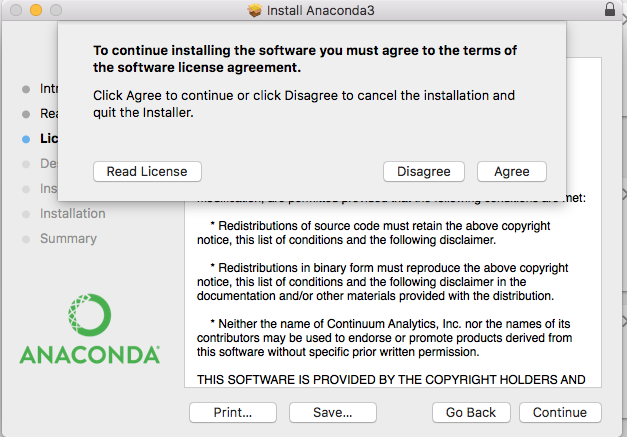
\includegraphics[scale=0.7]{Screenshot_6.png}}
\end{centering}

\paragraph{}
Choose who you want to install Anaconda for ("Install for me only" is fine).
\paragraph{}
\begin{centering}
    \centerline{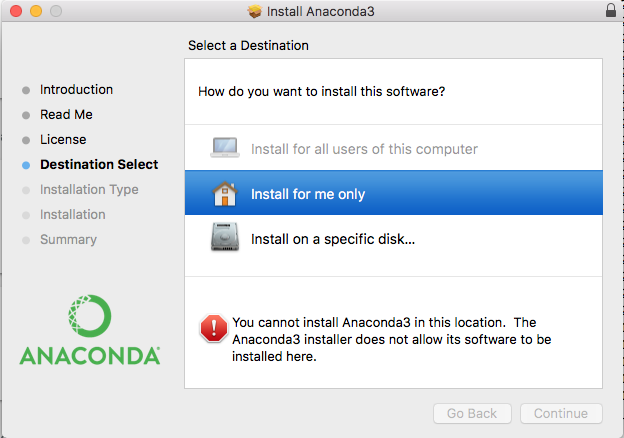
\includegraphics[scale=0.7]{Screenshot_7.png}}
\end{centering}

\paragraph{}
In the window below, you can choose where you want it to store Anaconda. The suggested (default) location is already filled in for you. Change the folder if you want to, then click Next.
\paragraph{}
\begin{centering}
    \centerline{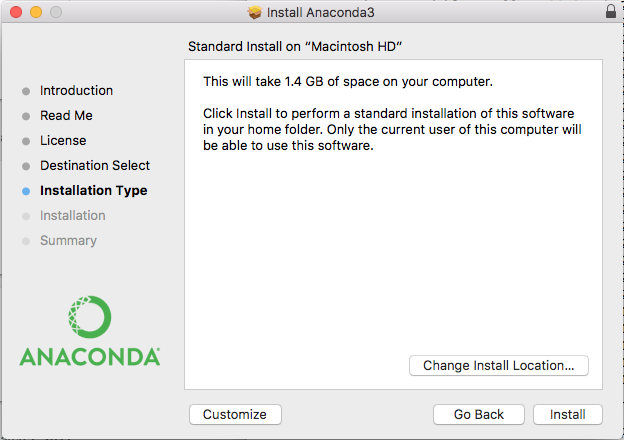
\includegraphics[scale=0.7]{Screenshot_8.png}}
\end{centering}
\paragraph{}

\paragraph{}
If you are asked for Advanced Installation Options (older version shown below), we recommend leaving both of these boxes checked. Then click Install.
\paragraph{}
\begin{centering}
    \centerline{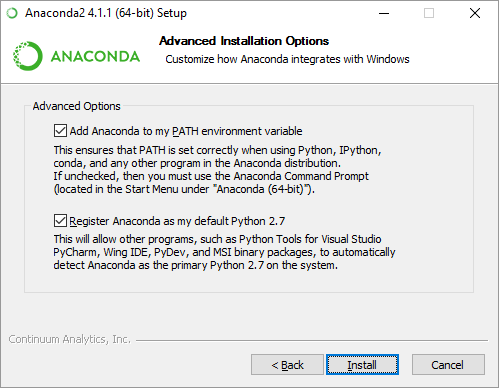
\includegraphics[scale=0.7]{Screenshot_9.png}}
\end{centering}

\paragraph{}
Wait for the program to install...
\paragraph{}
\begin{centering}
    \centerline{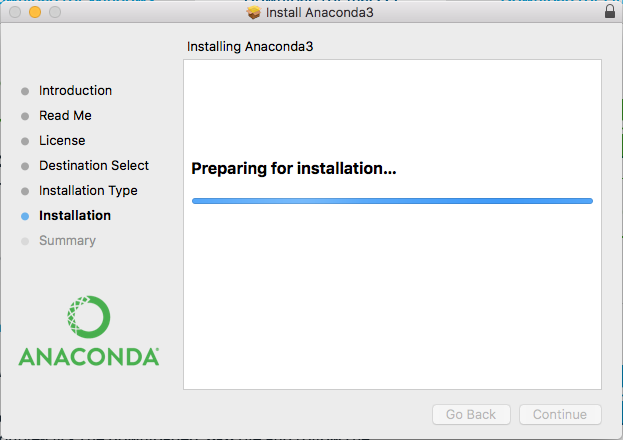
\includegraphics[scale=0.7]{Screenshot_10.png}}
\end{centering}

\paragraph{}
When it's finished, click Close. 
\paragraph{}
\begin{centering}
    \centerline{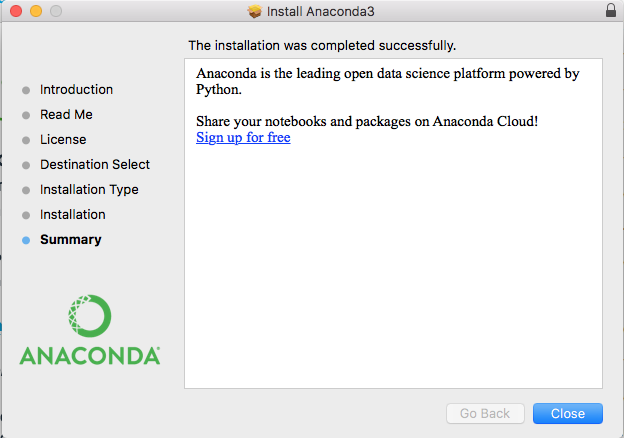
\includegraphics[scale=0.7]{Screenshot_11.png}}
\end{centering}

\paragraph{}
To launch Anaconda, search for "Anaconda-Navigator" in the Launchpad menu.
\paragraph{}
\begin{centering}
    \centerline{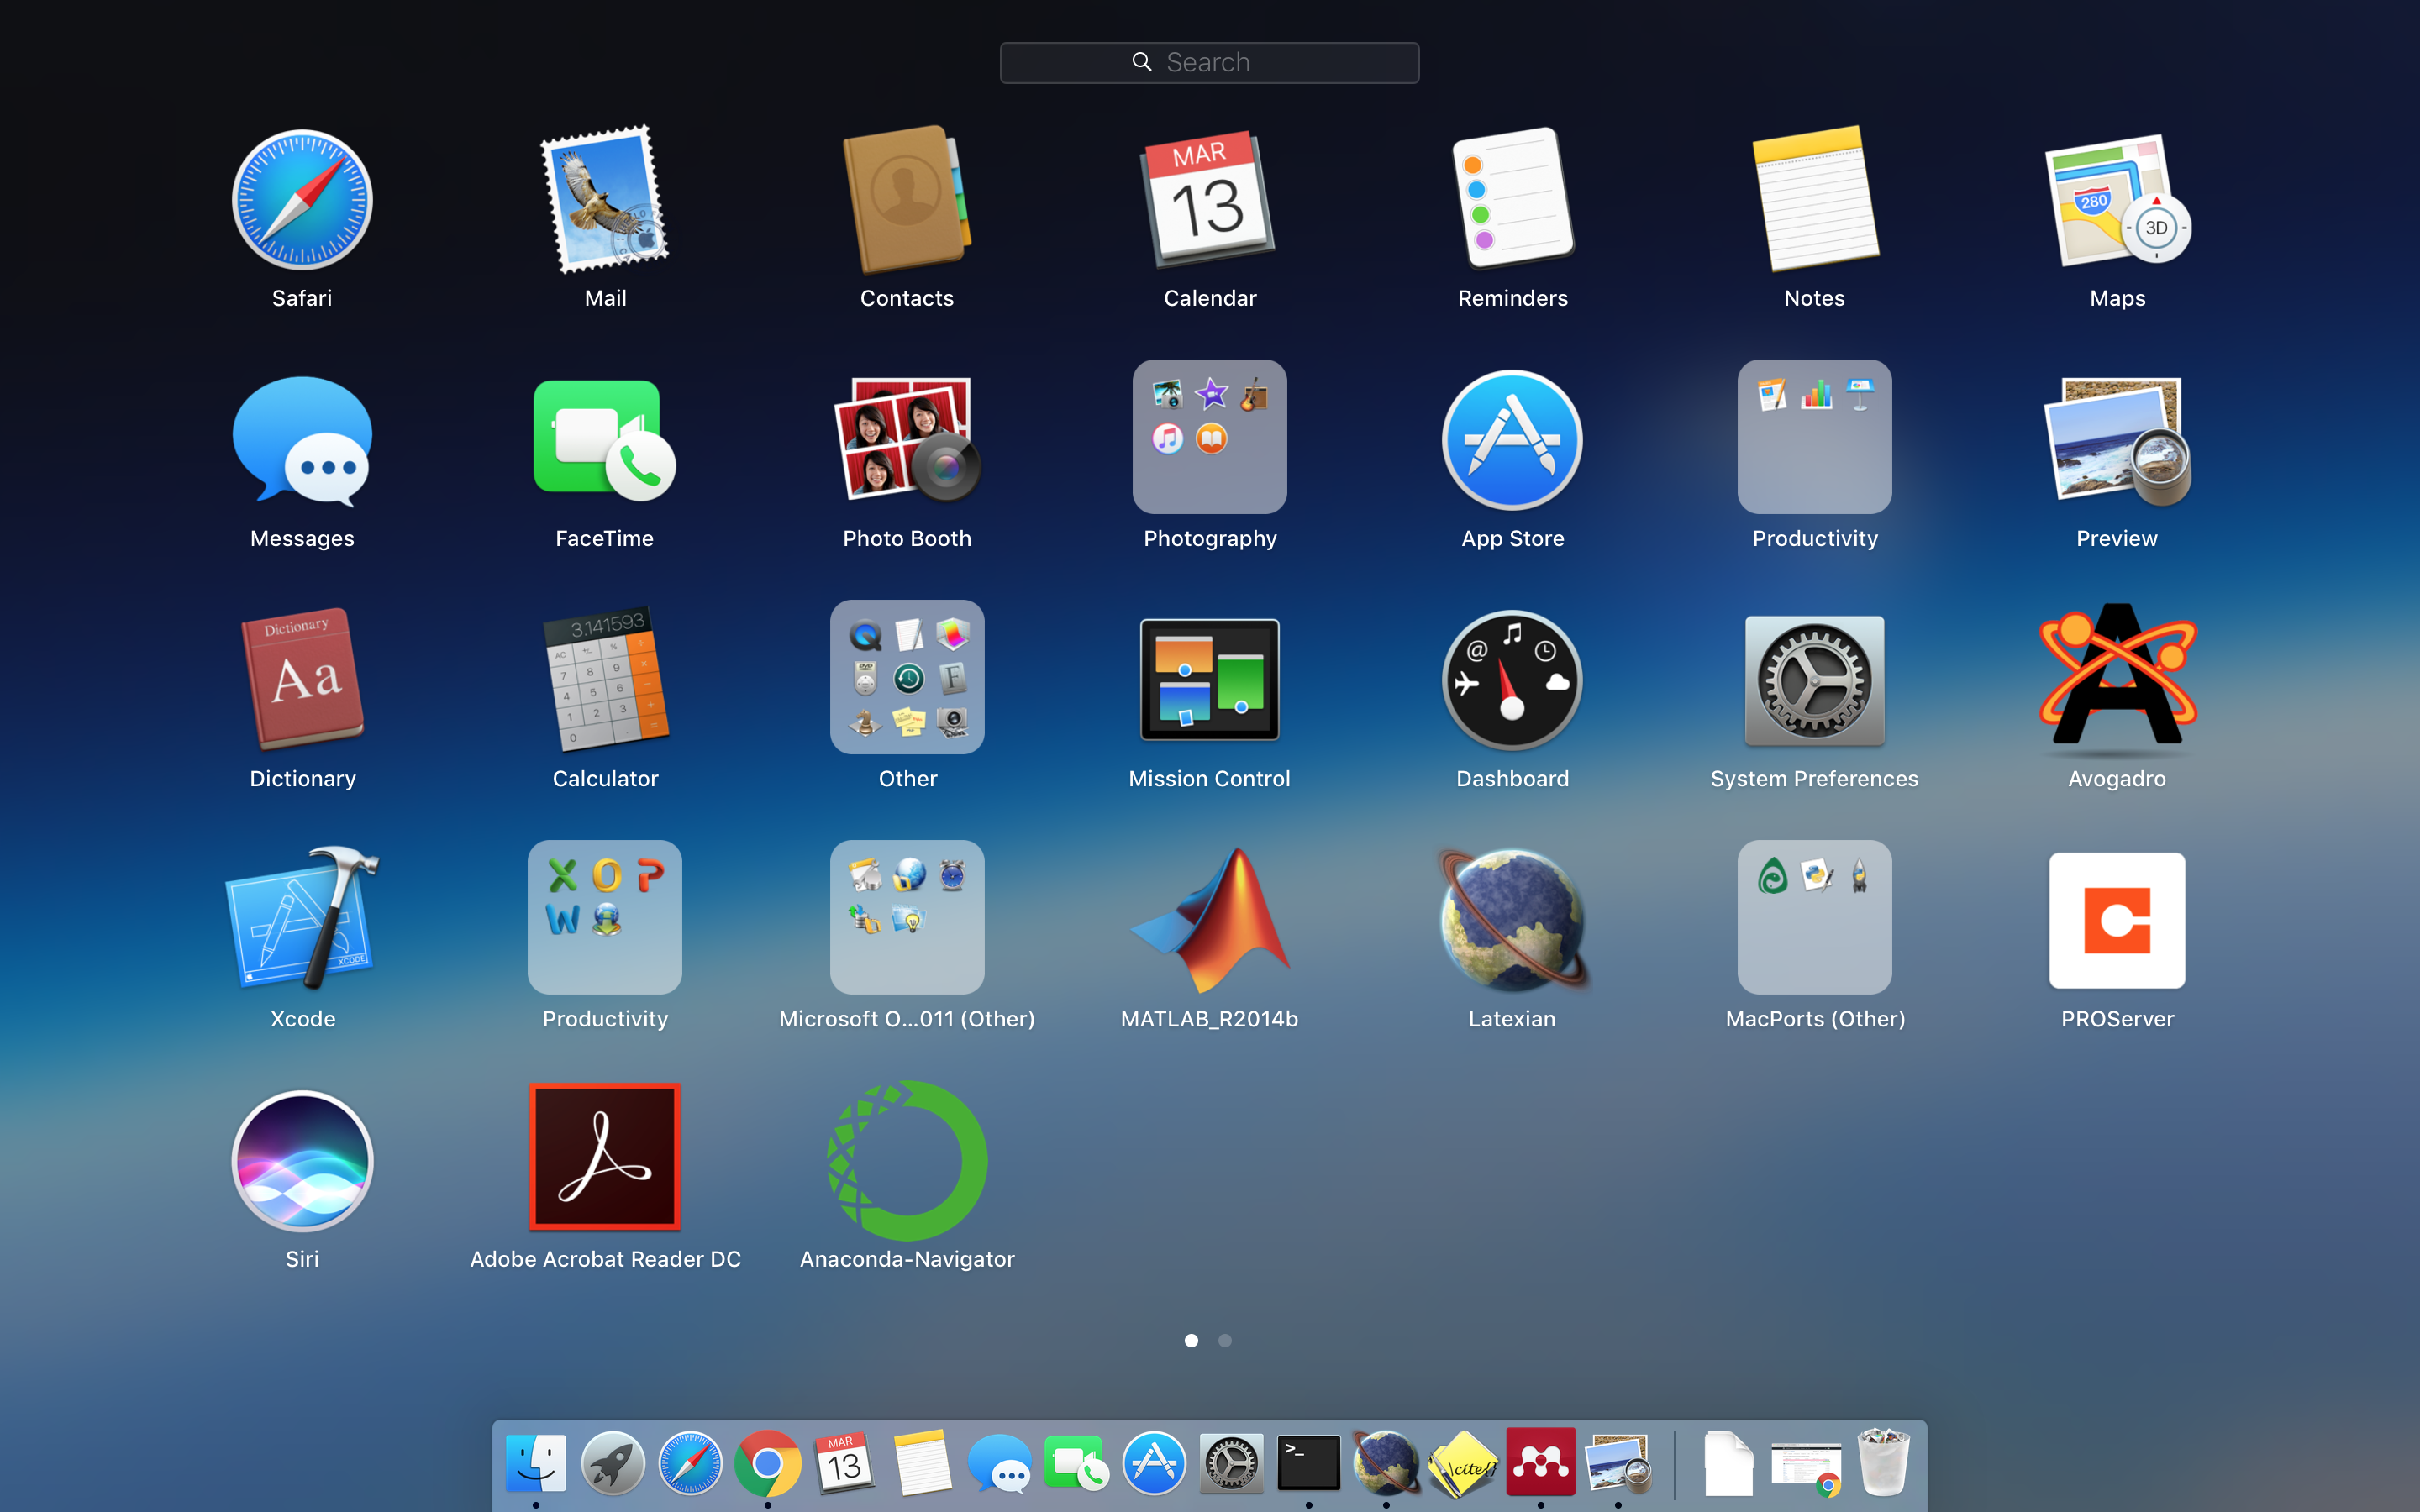
\includegraphics[scale=0.35]{Screenshot_13.png}}
\end{centering}

\paragraph{}
After the program launches, you should have a window that looks like the one below. For this workshop, we will only use one of the options here. Find the tile in the upper left named Jupyter Notebook, and click Launch.
\paragraph{}
\begin{centering}
    \centerline{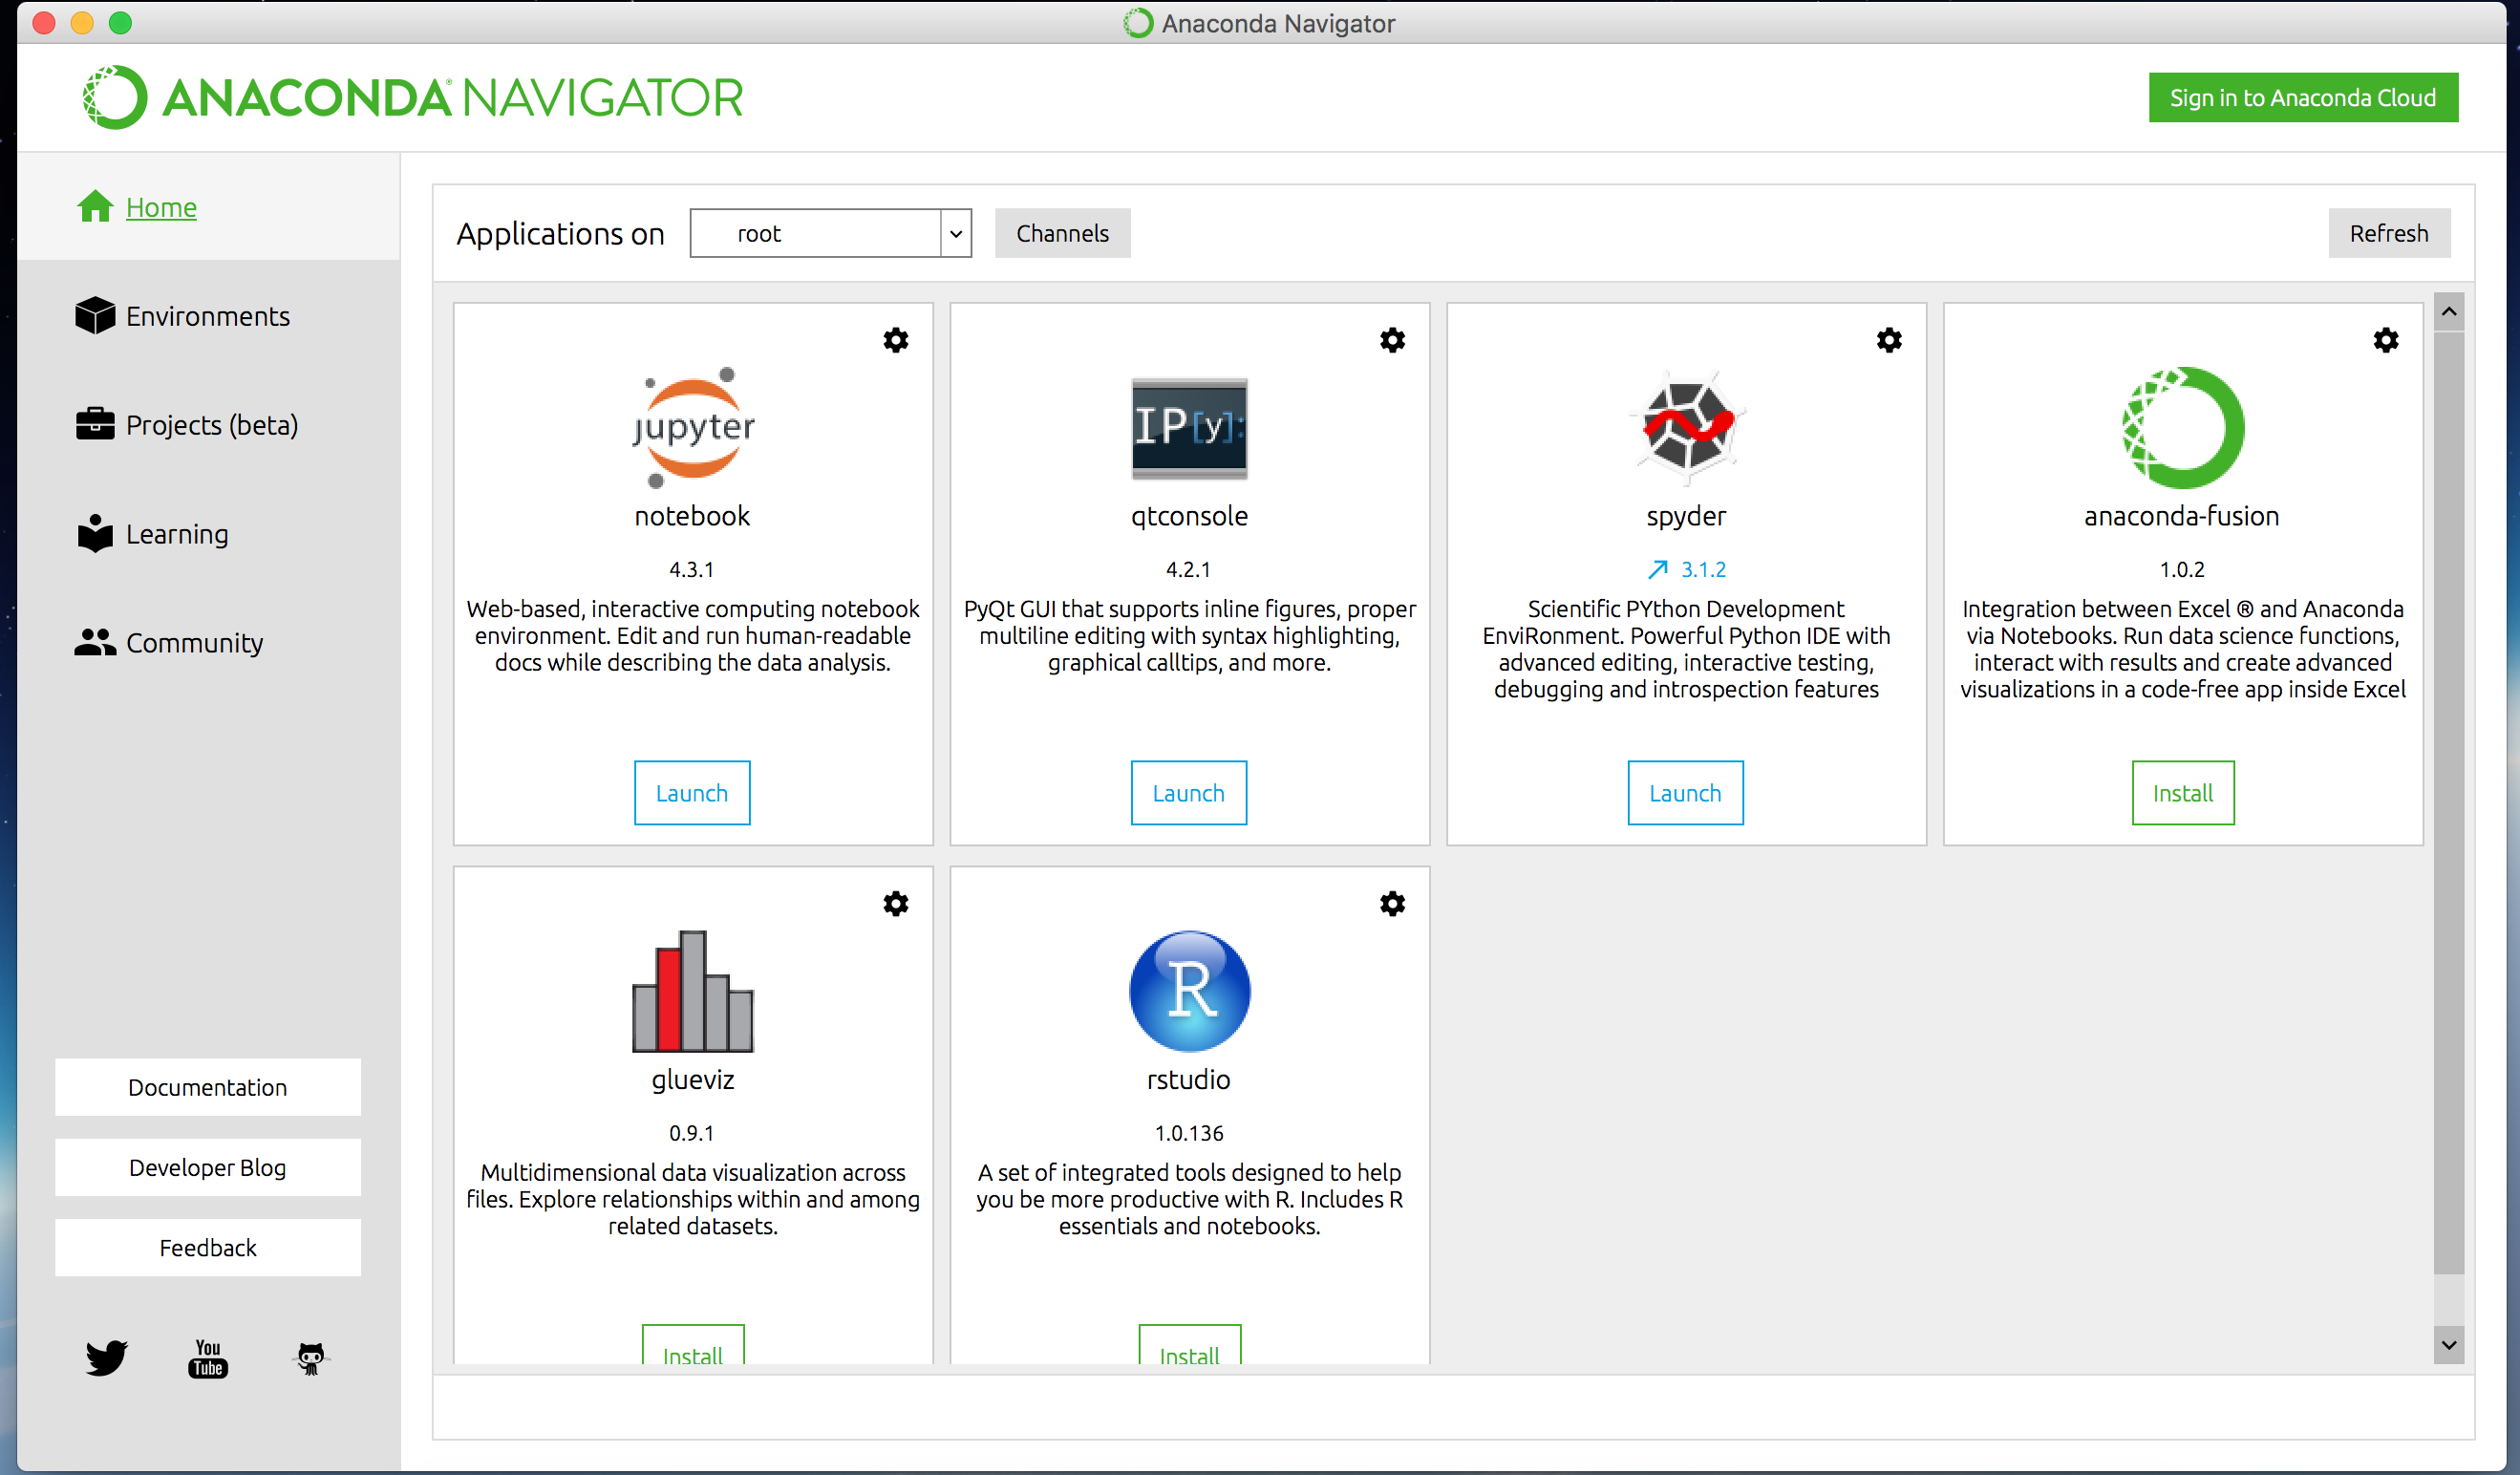
\includegraphics[scale=0.35]{Screenshot_14.png}}
\end{centering}

\paragraph{}
When the Jupyter notebook opens in your browser, you should get a screen looking something like this. The files and folders shown are what is on your own computer, so those will look different from the example. We recommend creating a folder where you can store and edit your Python work. To do this, click on the word New in the upper right corner, and choose Folder.
\paragraph{}
\begin{centering}
    \centerline{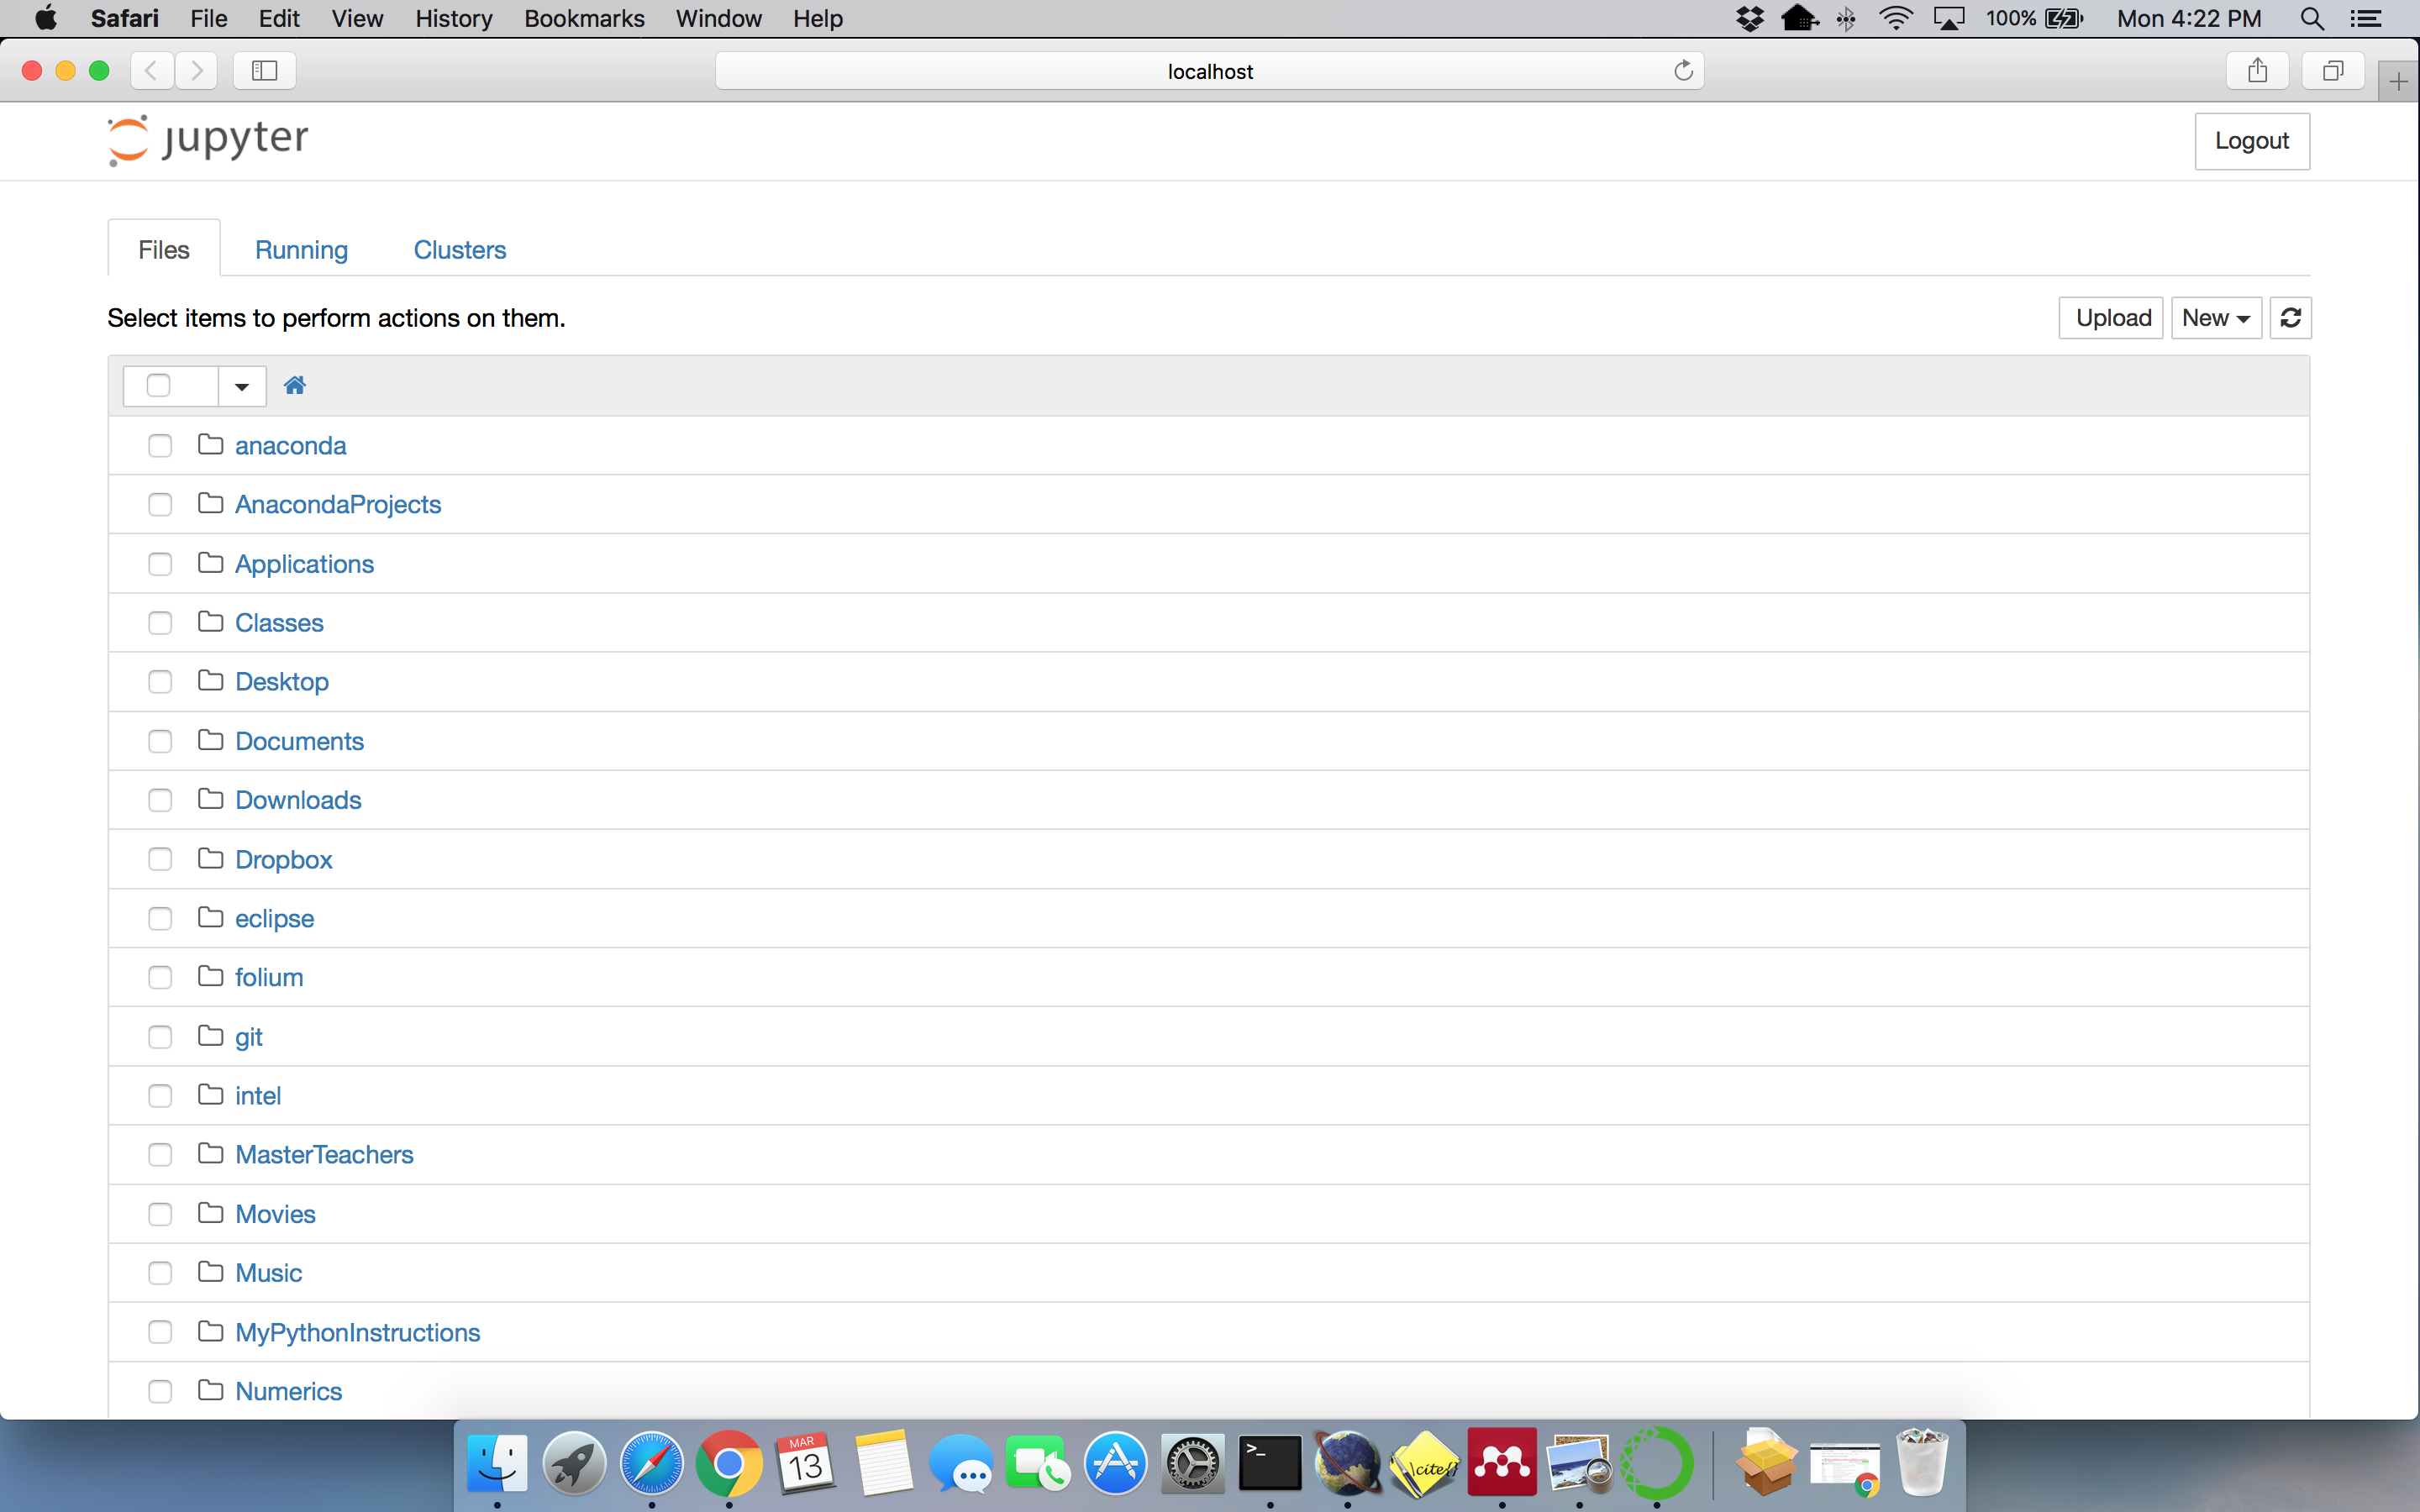
\includegraphics[scale=0.35]{Screenshot_16.png}}
\end{centering}

\paragraph{}
This will create an Untitled folder in the window. To change the name of the folder, check the box next to the Untitled folder, then click Rename at the top of the window (you may have to scroll down to see the Untitled folder, and then back up to see the Rename button).
\paragraph{}
\begin{centering}
    \centerline{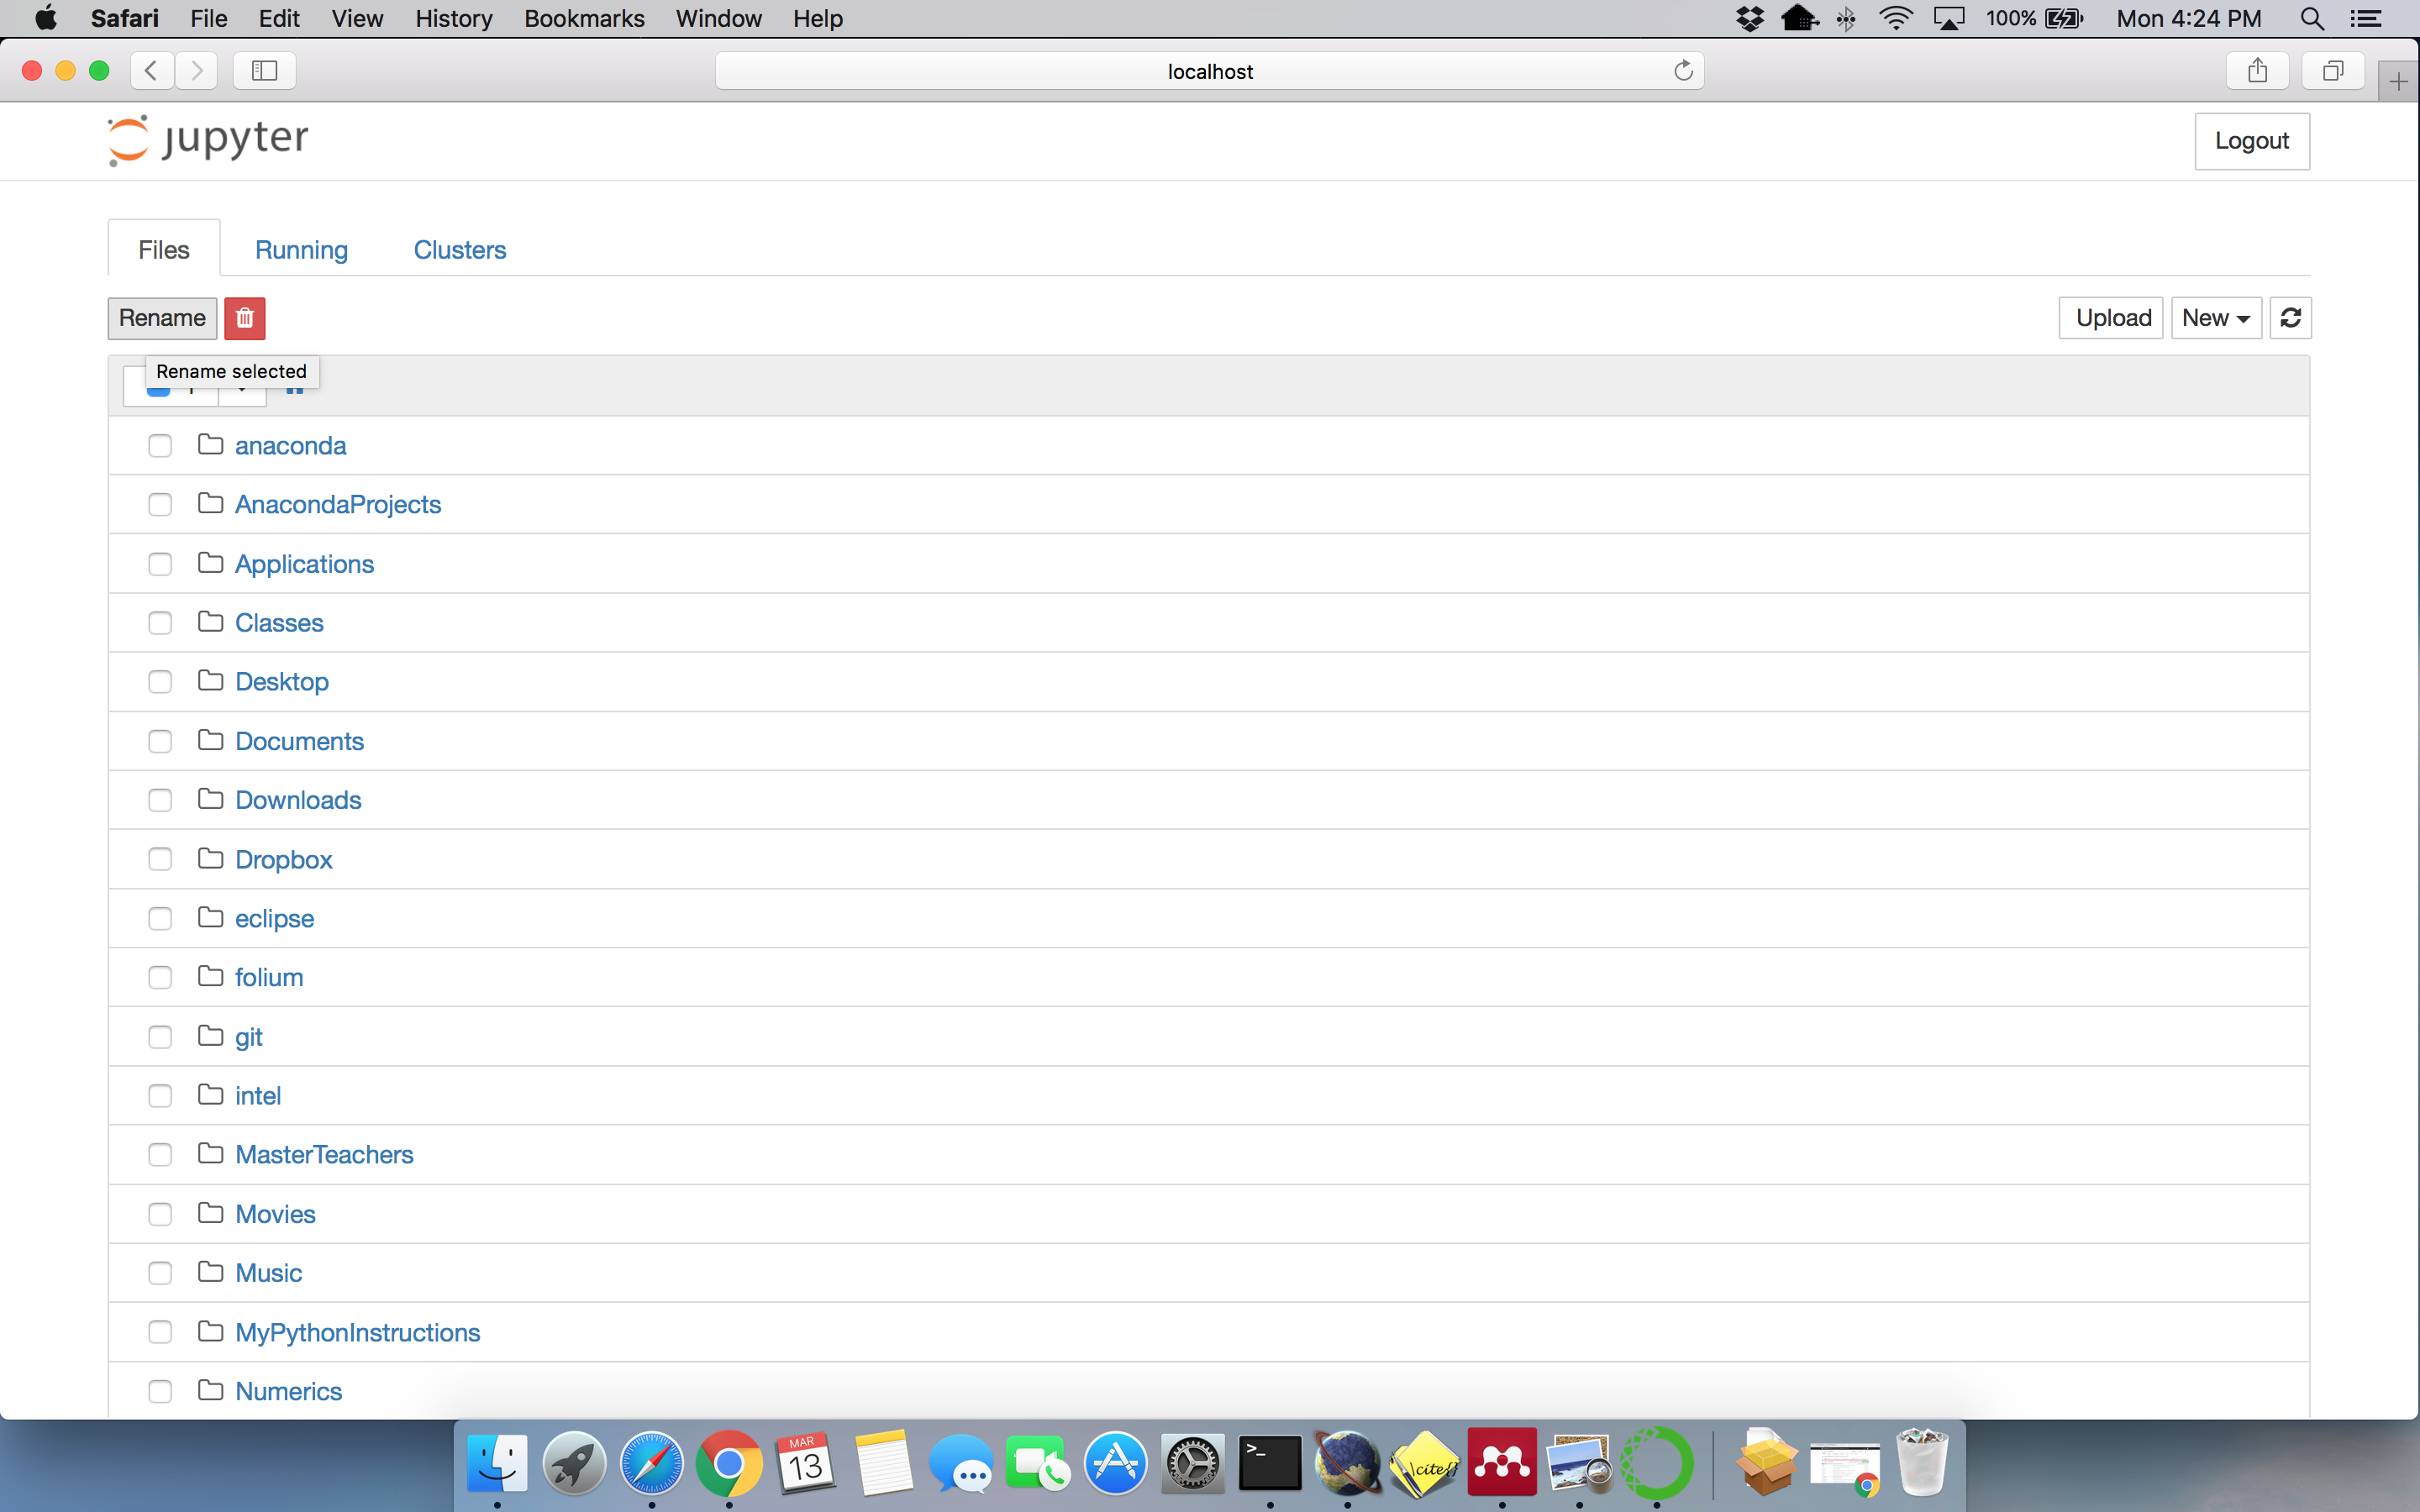
\includegraphics[scale=0.35]{Screenshot_18.png}}
\end{centering}

\paragraph{}
You can type whatever name you want into the box prompt. We simply named ours Python. After you've created your folder, click on the folder name to go into the folder.
\paragraph{}
\begin{centering}
    \centerline{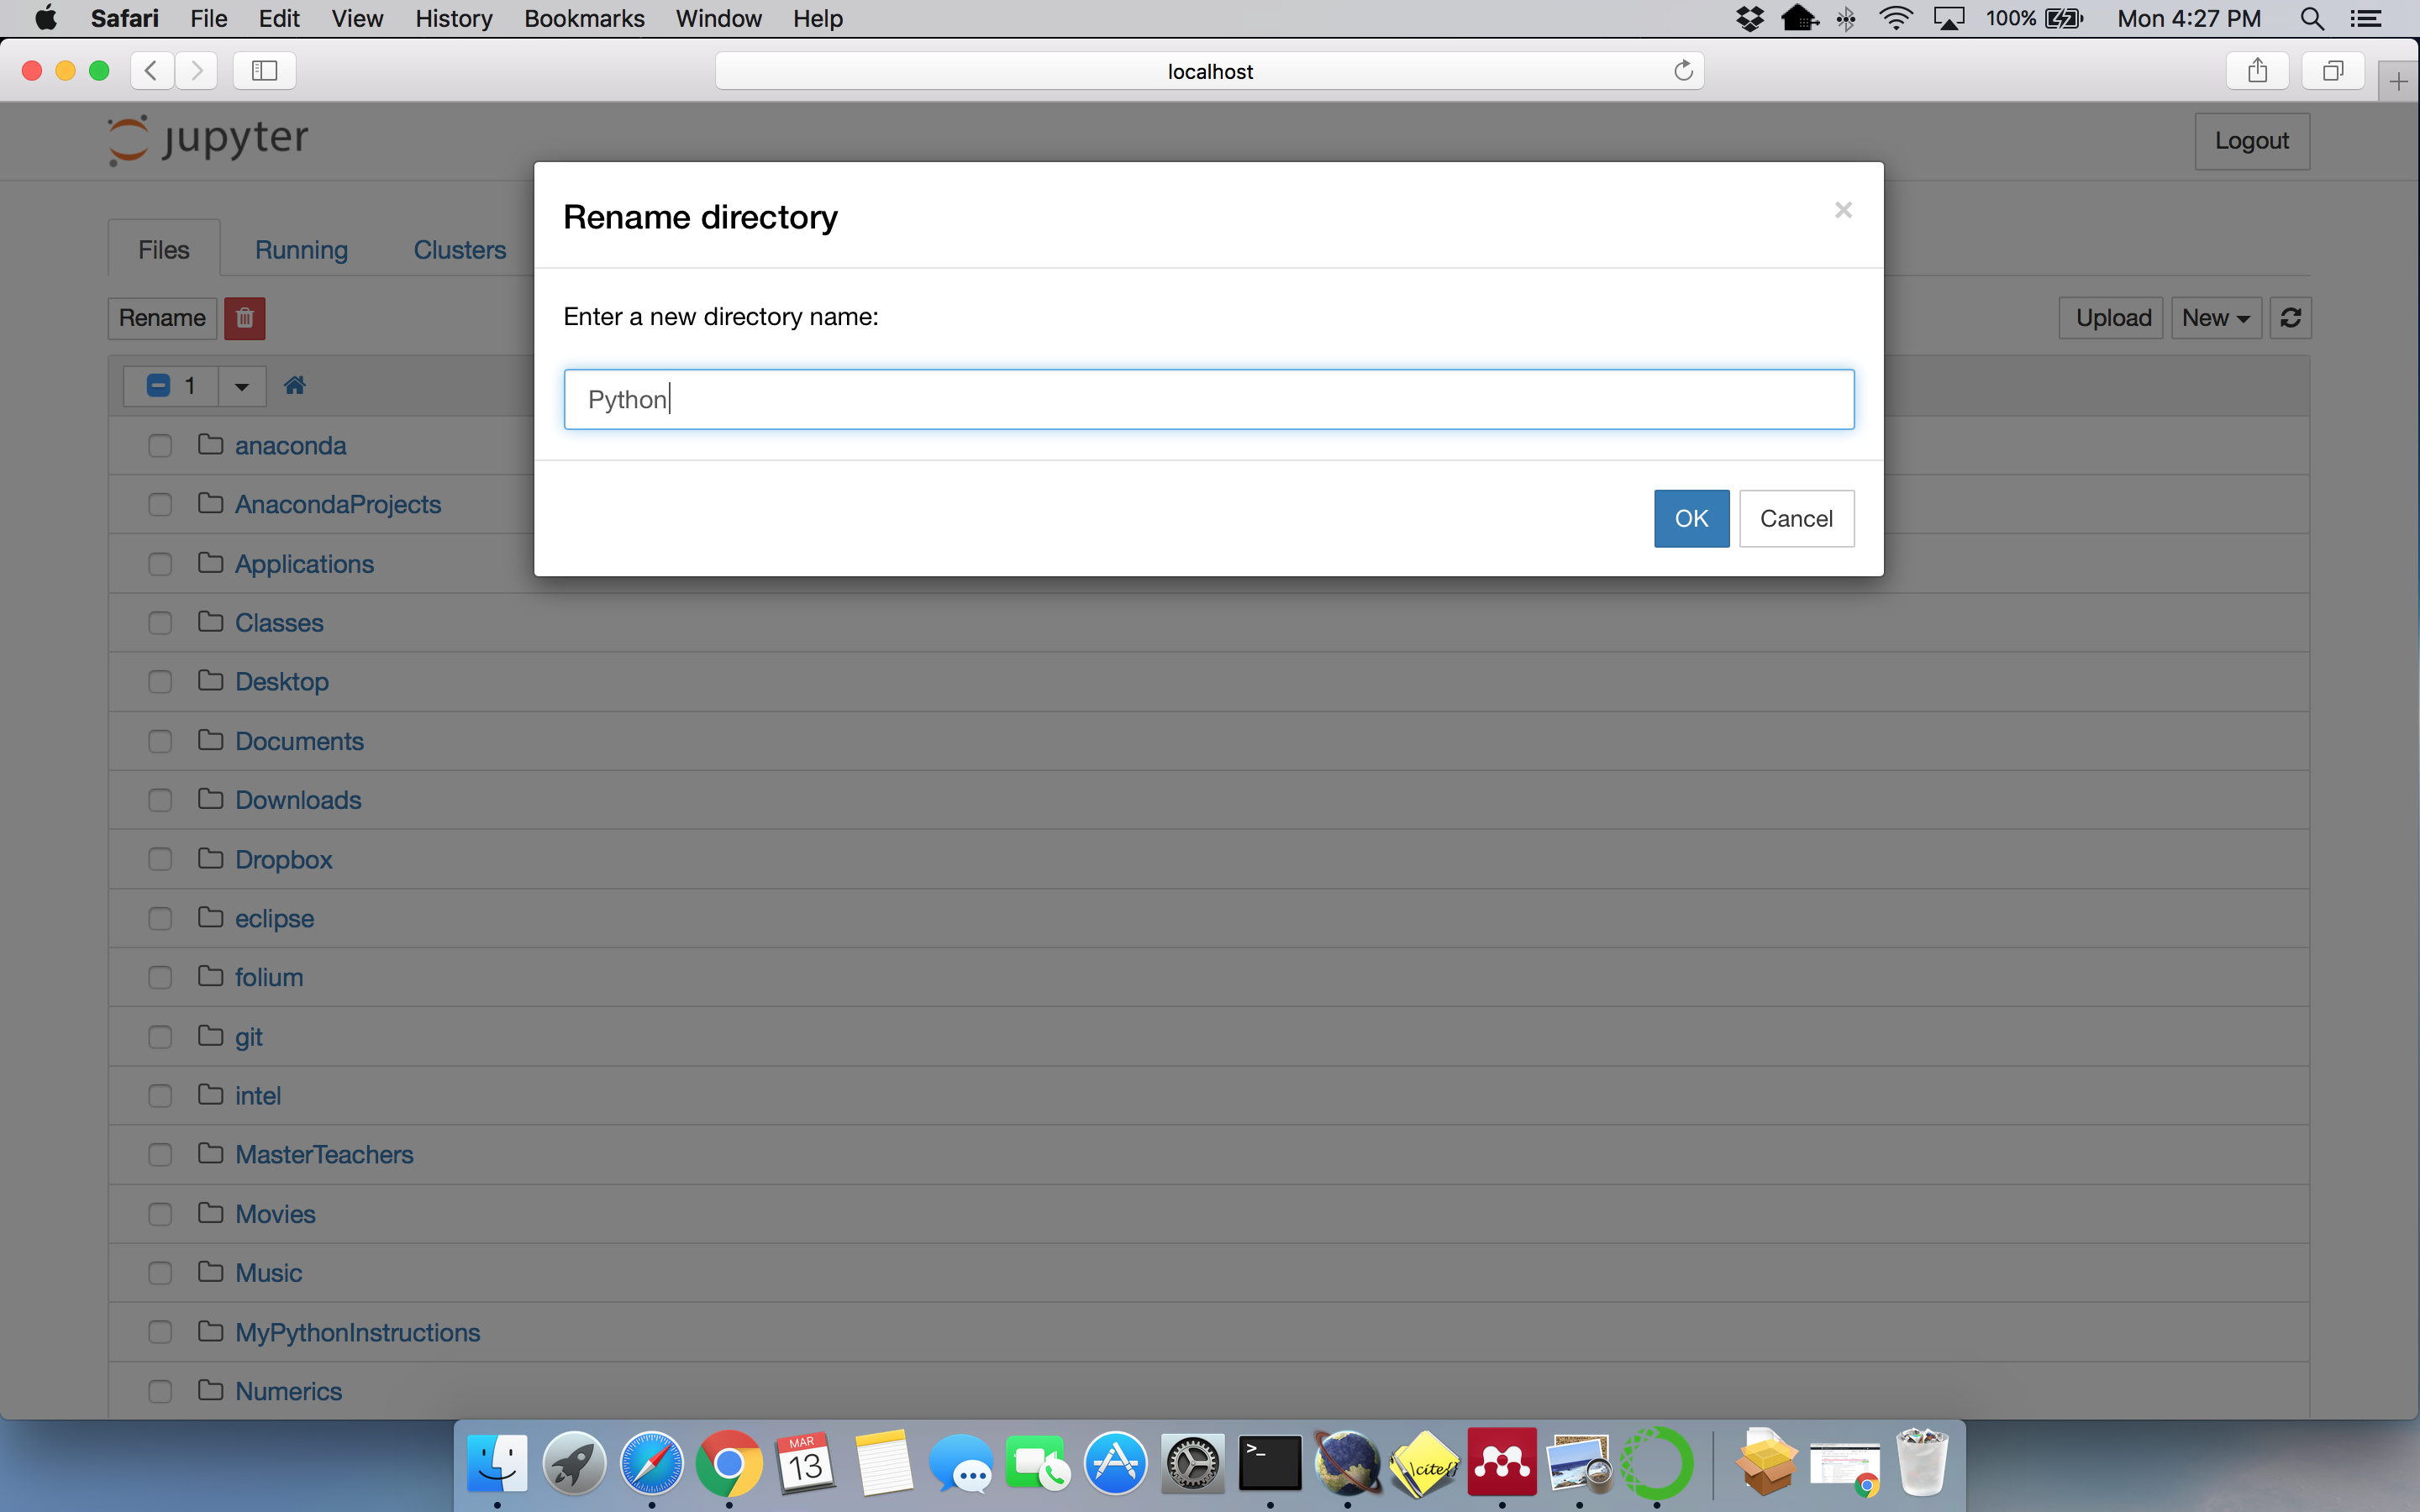
\includegraphics[scale=0.35]{Screenshot_19.png}}
\end{centering}

\paragraph{}
You should have a screen that looks something like this. Now let's create our first Notebook. Click on New, then click on Python [Root] (Your computer may say Python 3 instead of Python [Root])
\paragraph{}
\begin{centering}
    \centerline{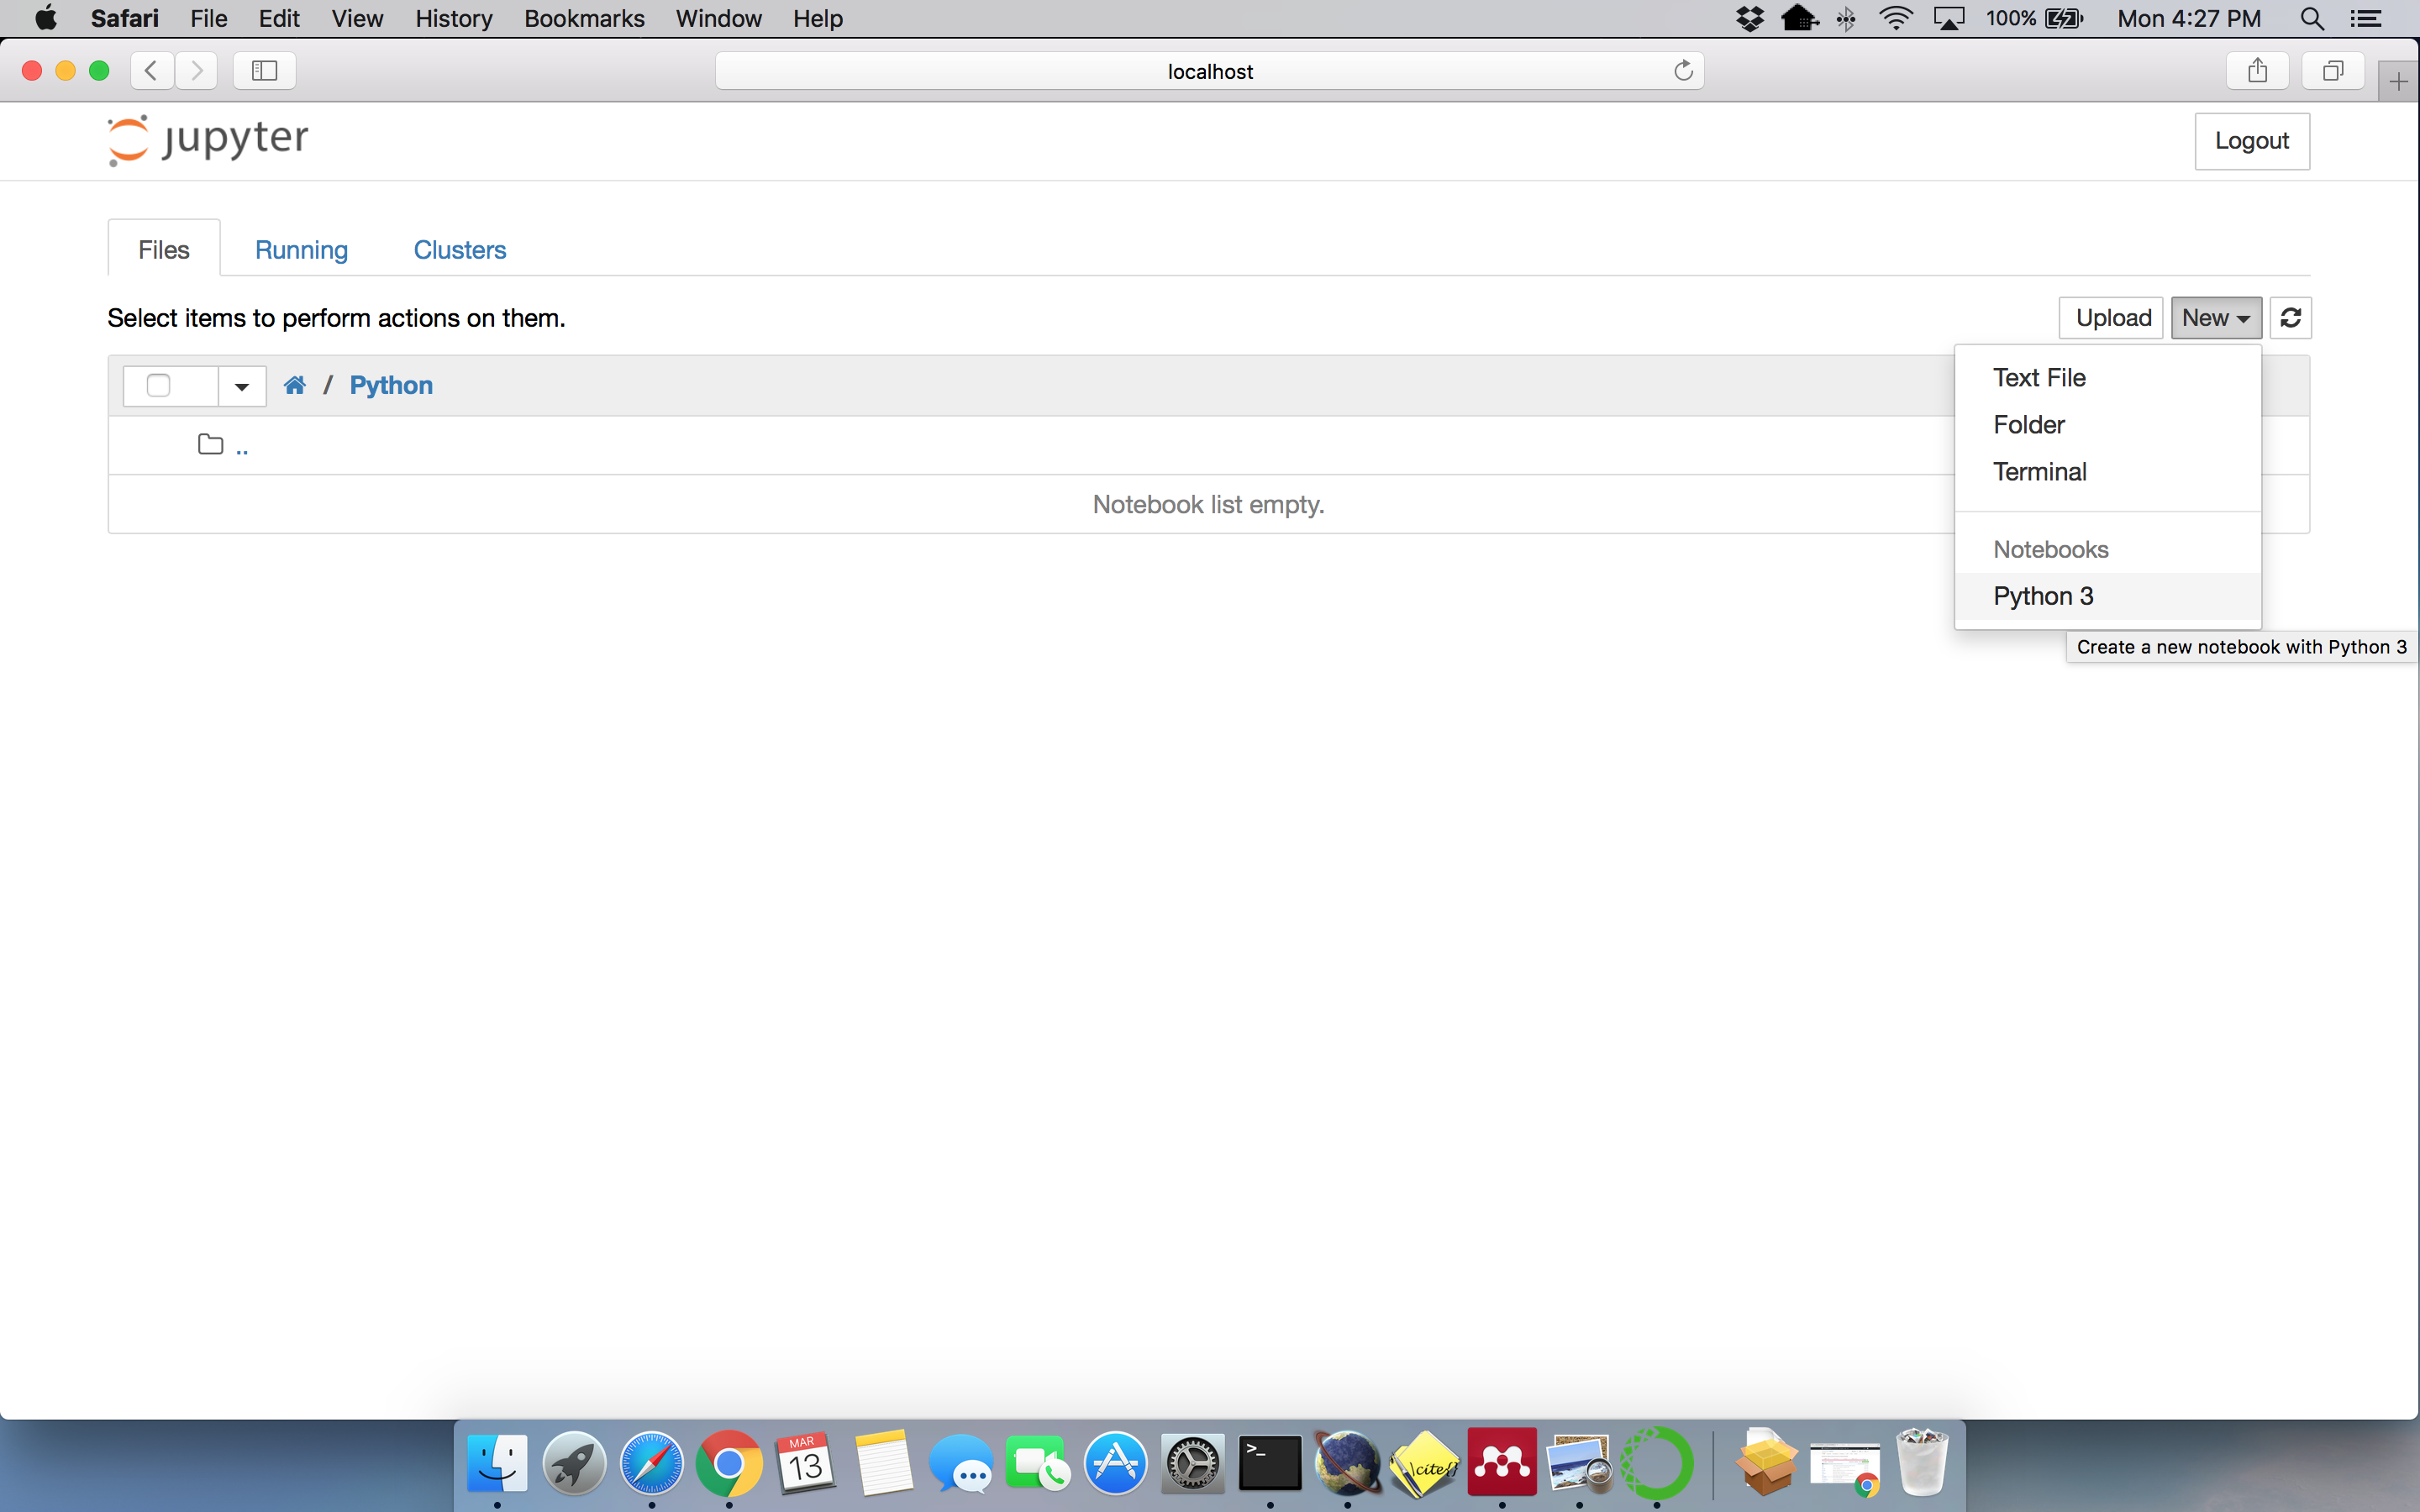
\includegraphics[scale=0.35]{Screenshot_20.png}}
\end{centering}

\paragraph{}
This should open a blank notebook. The computer automatically gives you an empty box to type in called a "cell." What you type in the cell depends on the kind of cell you're given. One of the most important features of the notebook is the dropdown menu at the top, as shown in the picture below. This changes the selected cell to the kind of your choice. We will only use "Code" and "Markdown" cells for this workshop. A Markdown cell can be thought of just normal text. When you type in a markdown cell, it's just like typing in any other text editor. A Code cell is what we use to type code that we want the computer to execute. For now, let's leave this set to "Code."
\paragraph{}
\begin{centering}
    \centerline{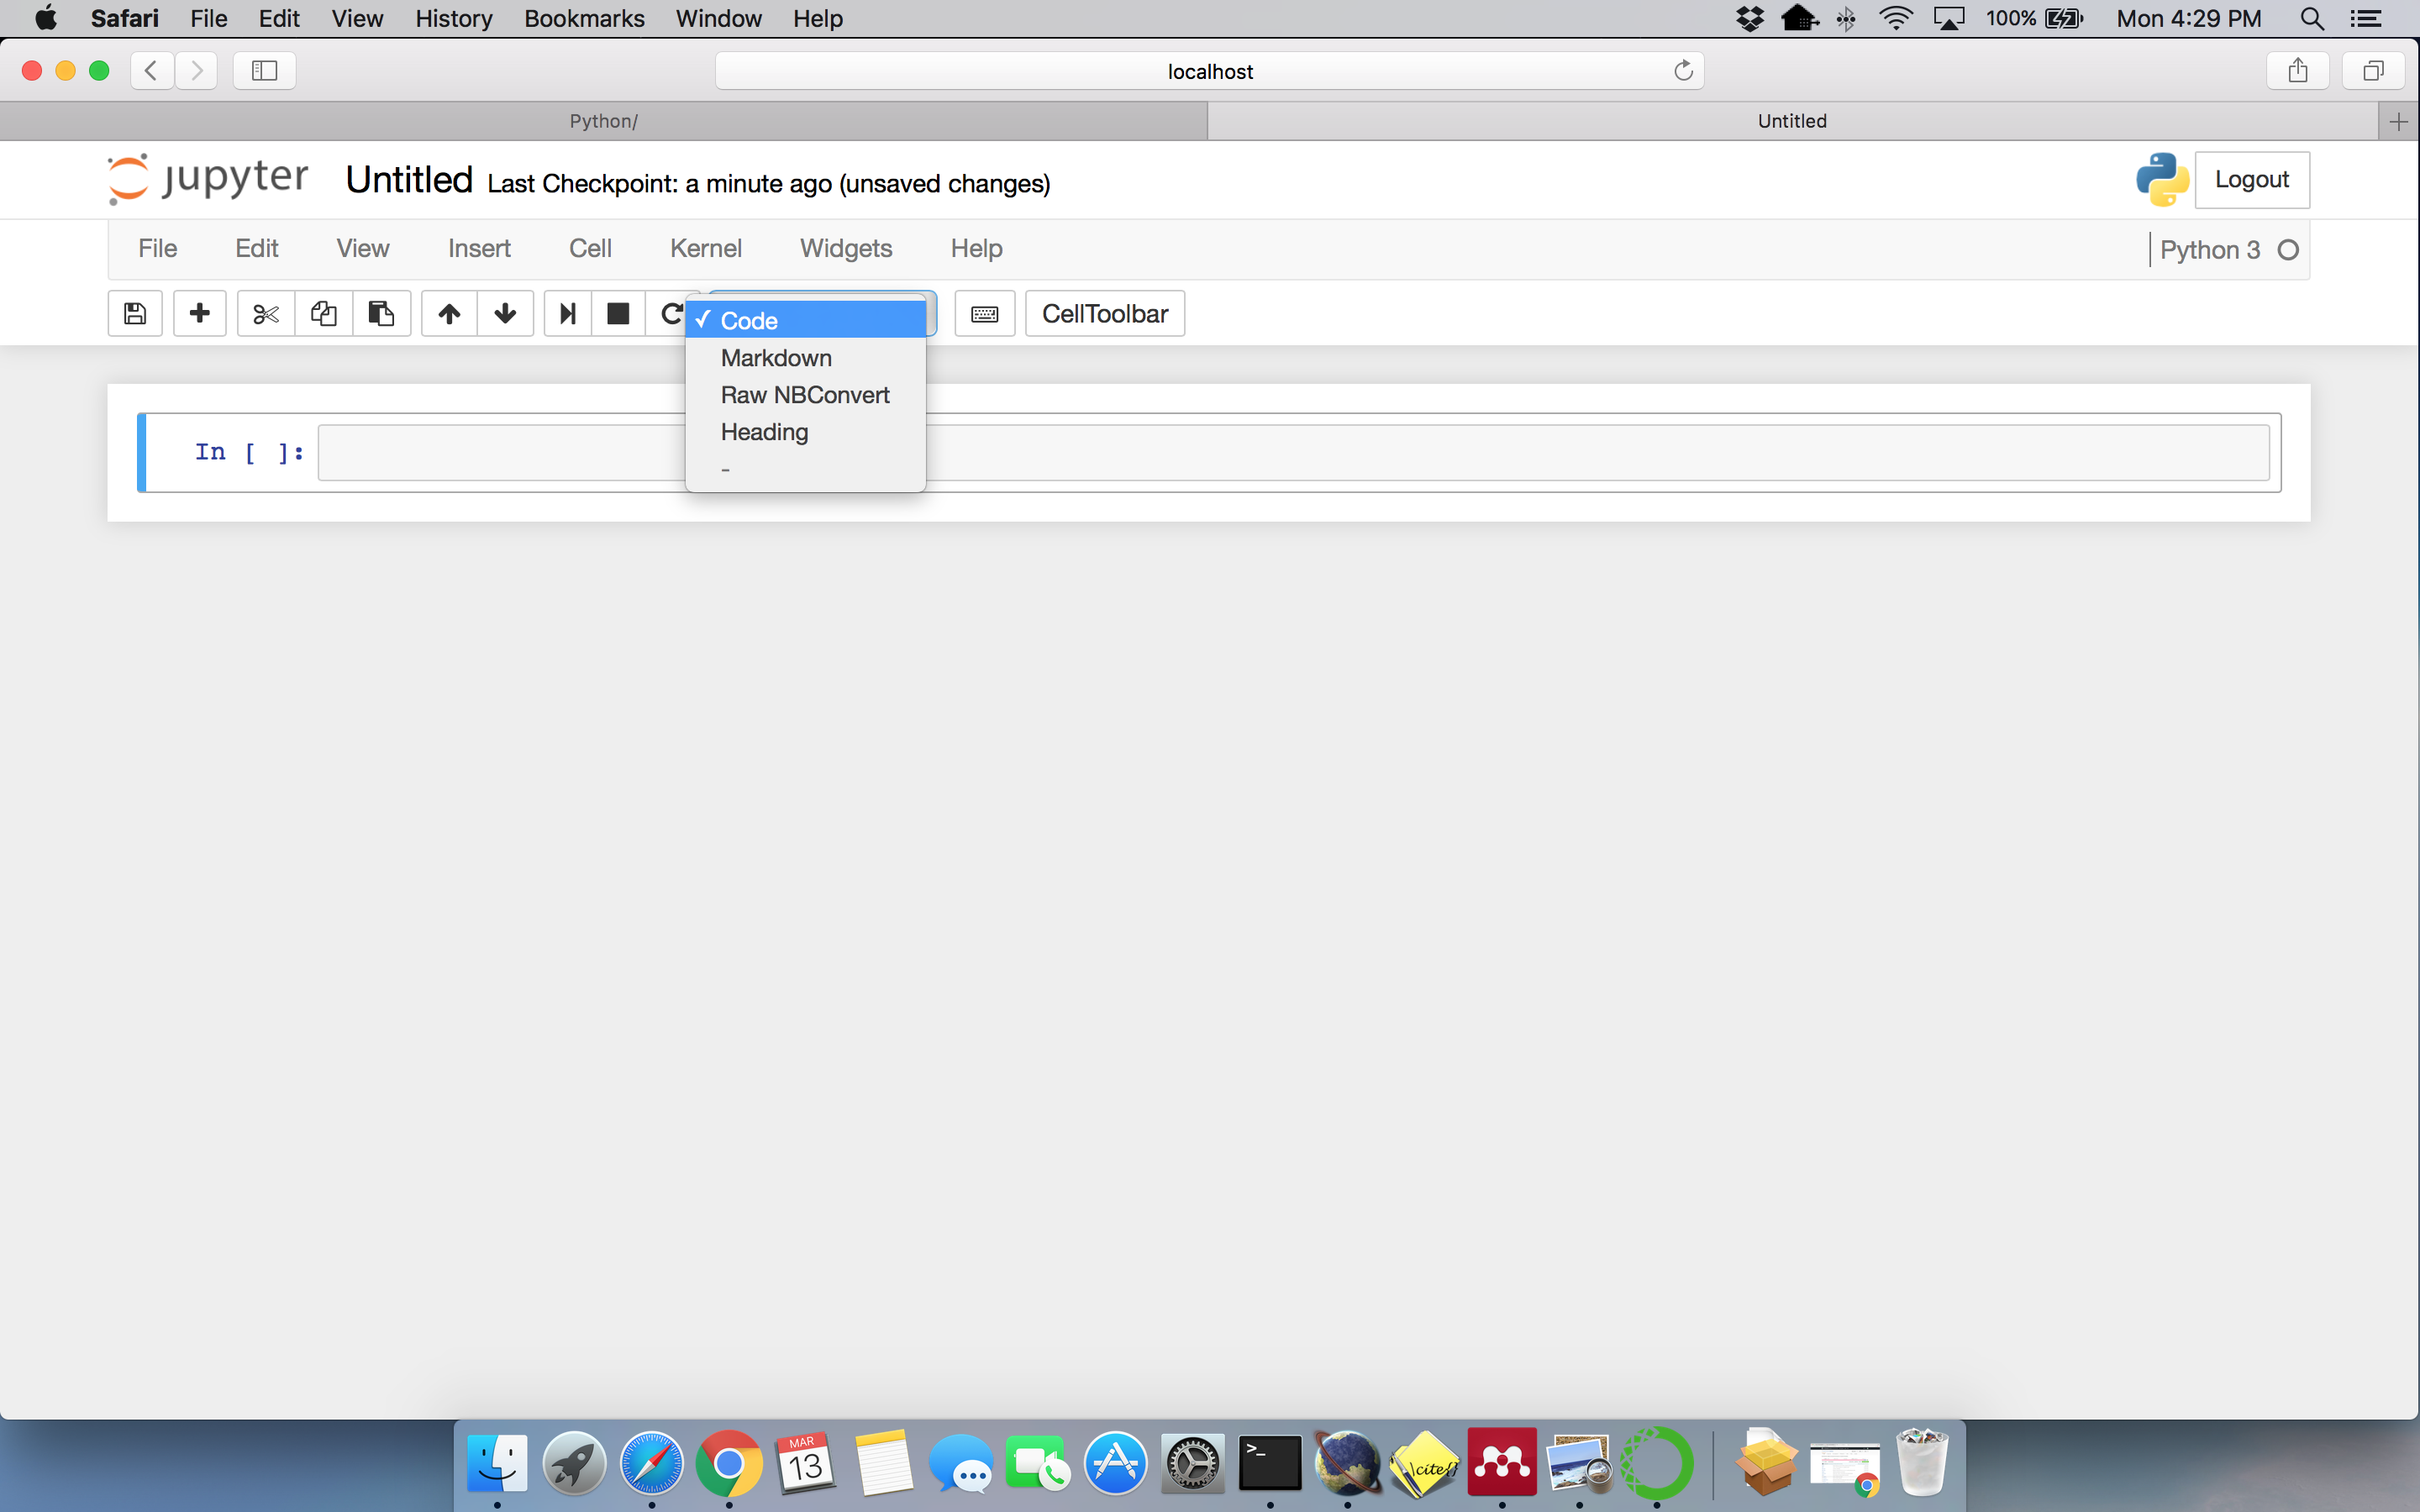
\includegraphics[scale=0.35]{Screenshot_21.png}}
\end{centering}

\paragraph{}
You can name your notebook by clicking on the title at the top (Currently the title is "Untitled"). Feel free to name this whatever you please. Then click OK.
\paragraph{}
\begin{centering}
    \centerline{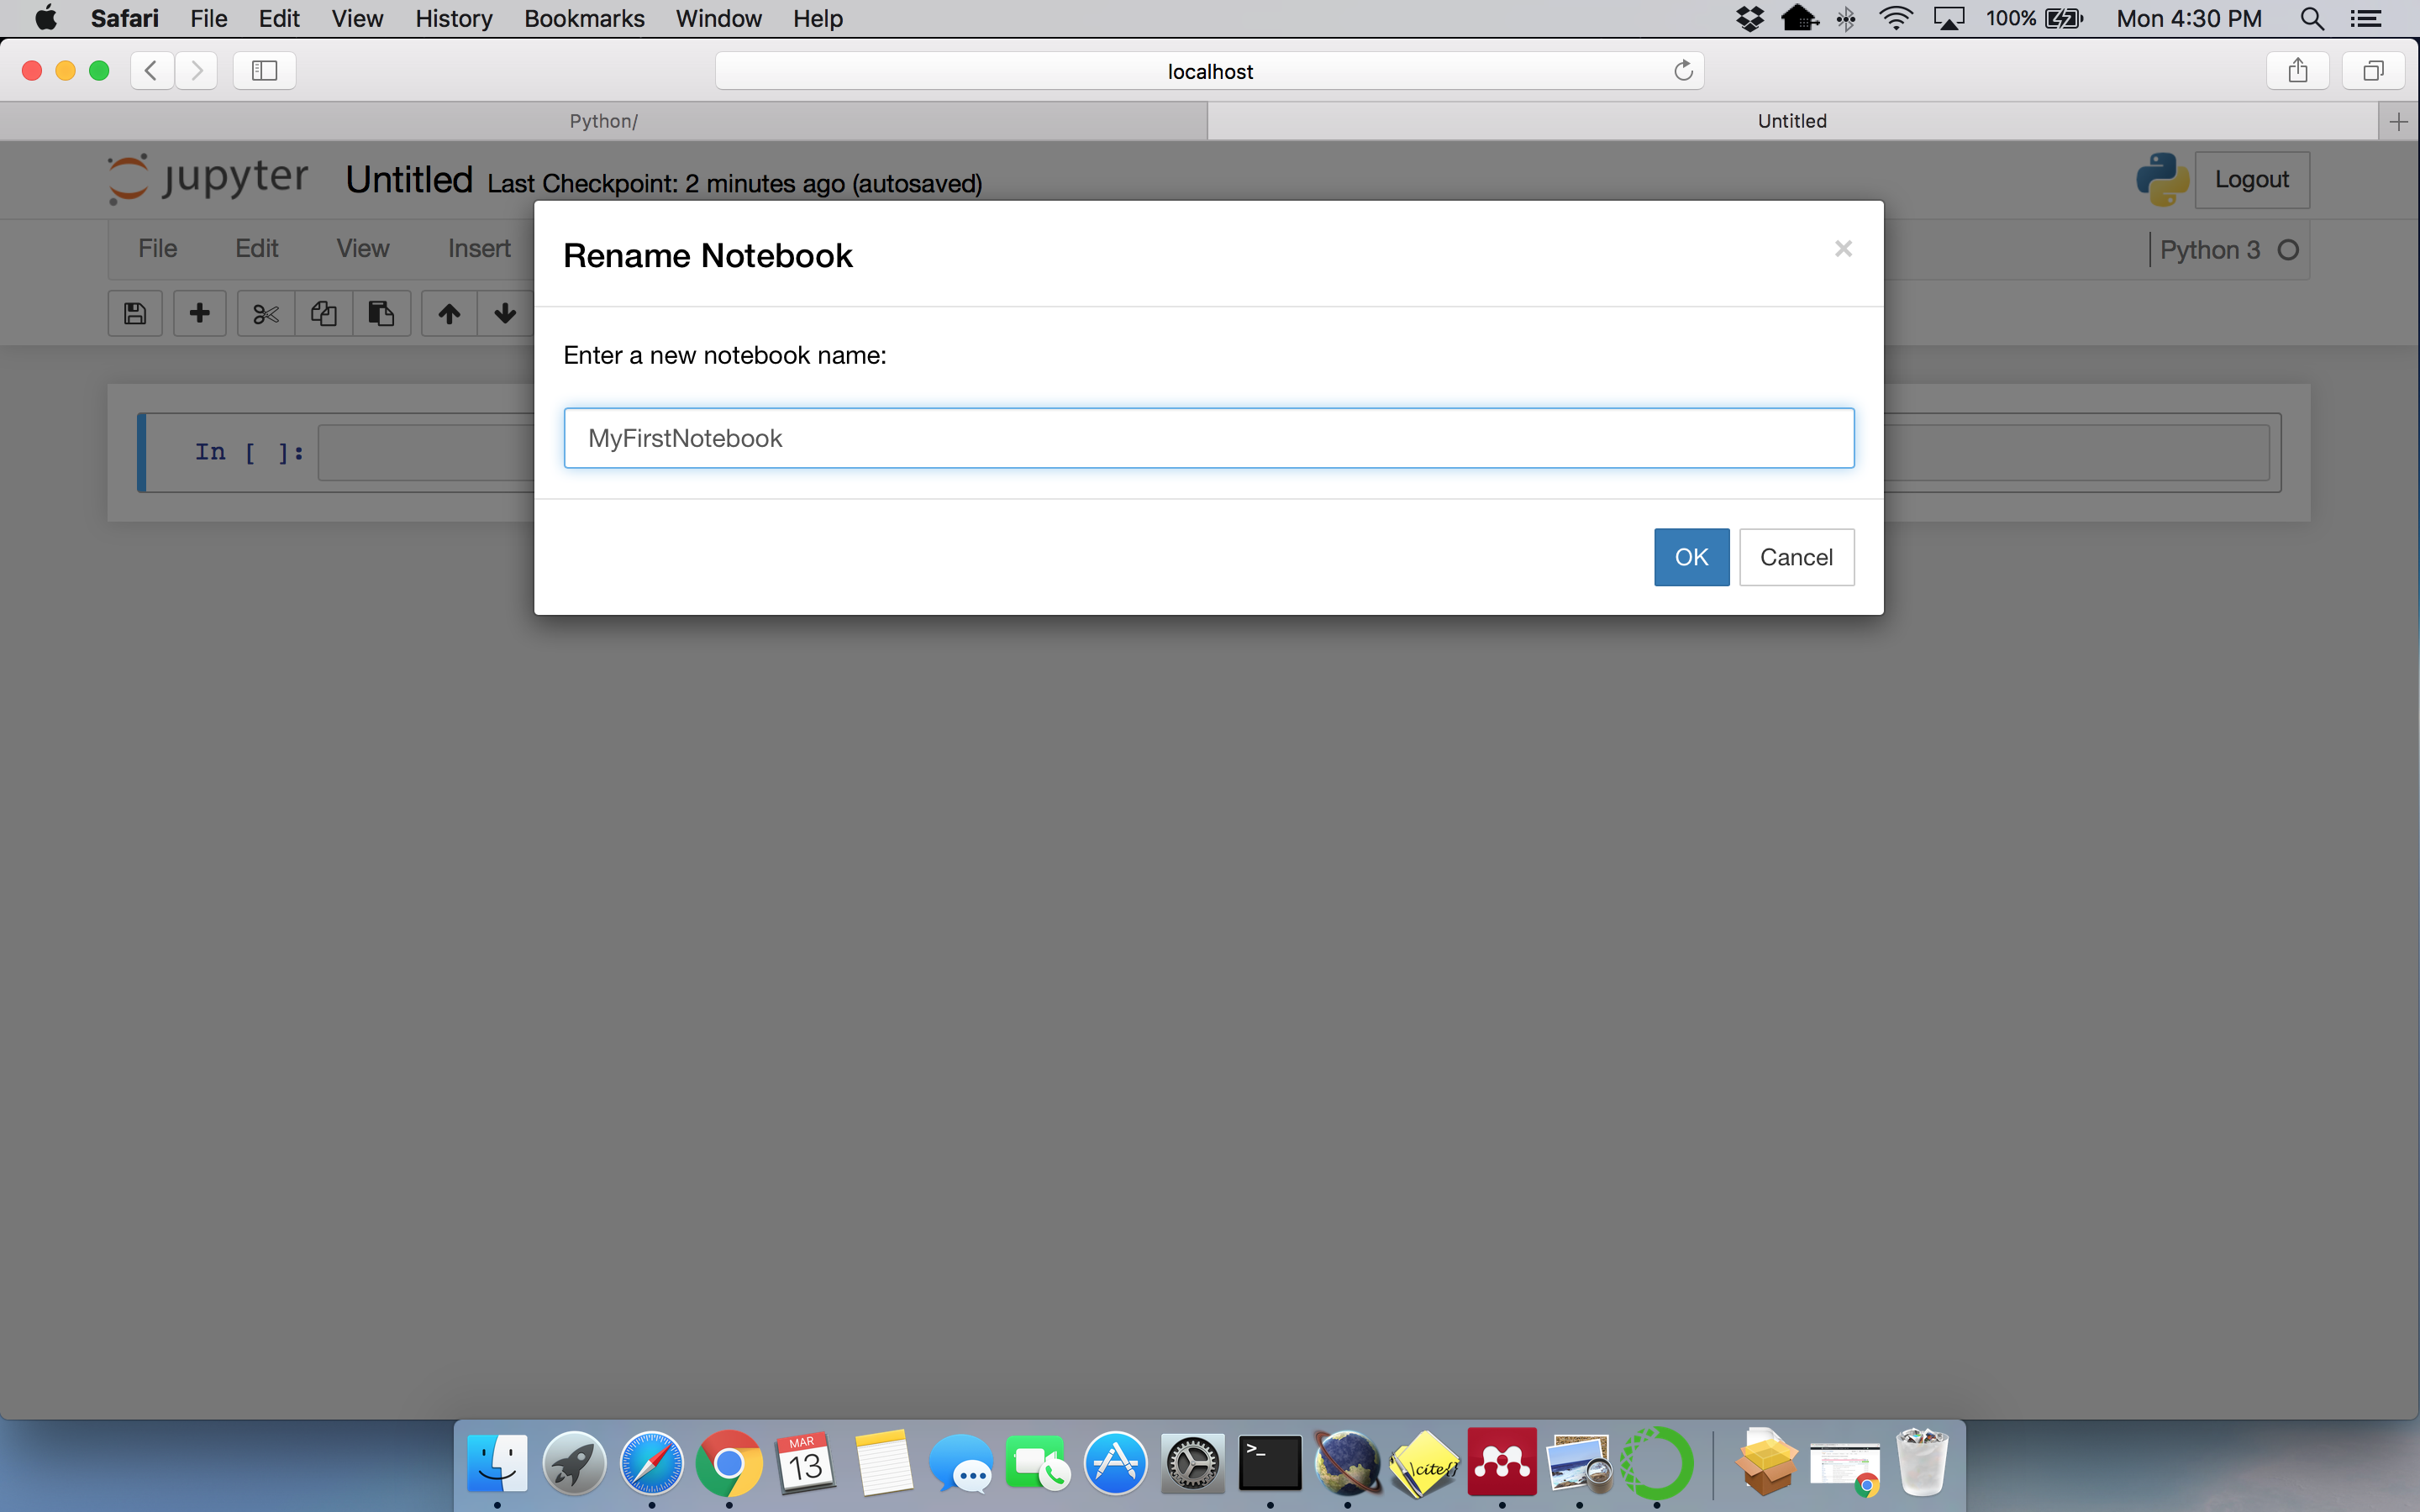
\includegraphics[scale=0.35]{Screenshot_22.png}}
\end{centering}

\paragraph{}
If you want to try your hand at some Python, type in the first cell the command shown in the picture below. Be careful: the text on your screen should read exactly as it does in the picture below.
\paragraph{}
\begin{centering}
    \centerline{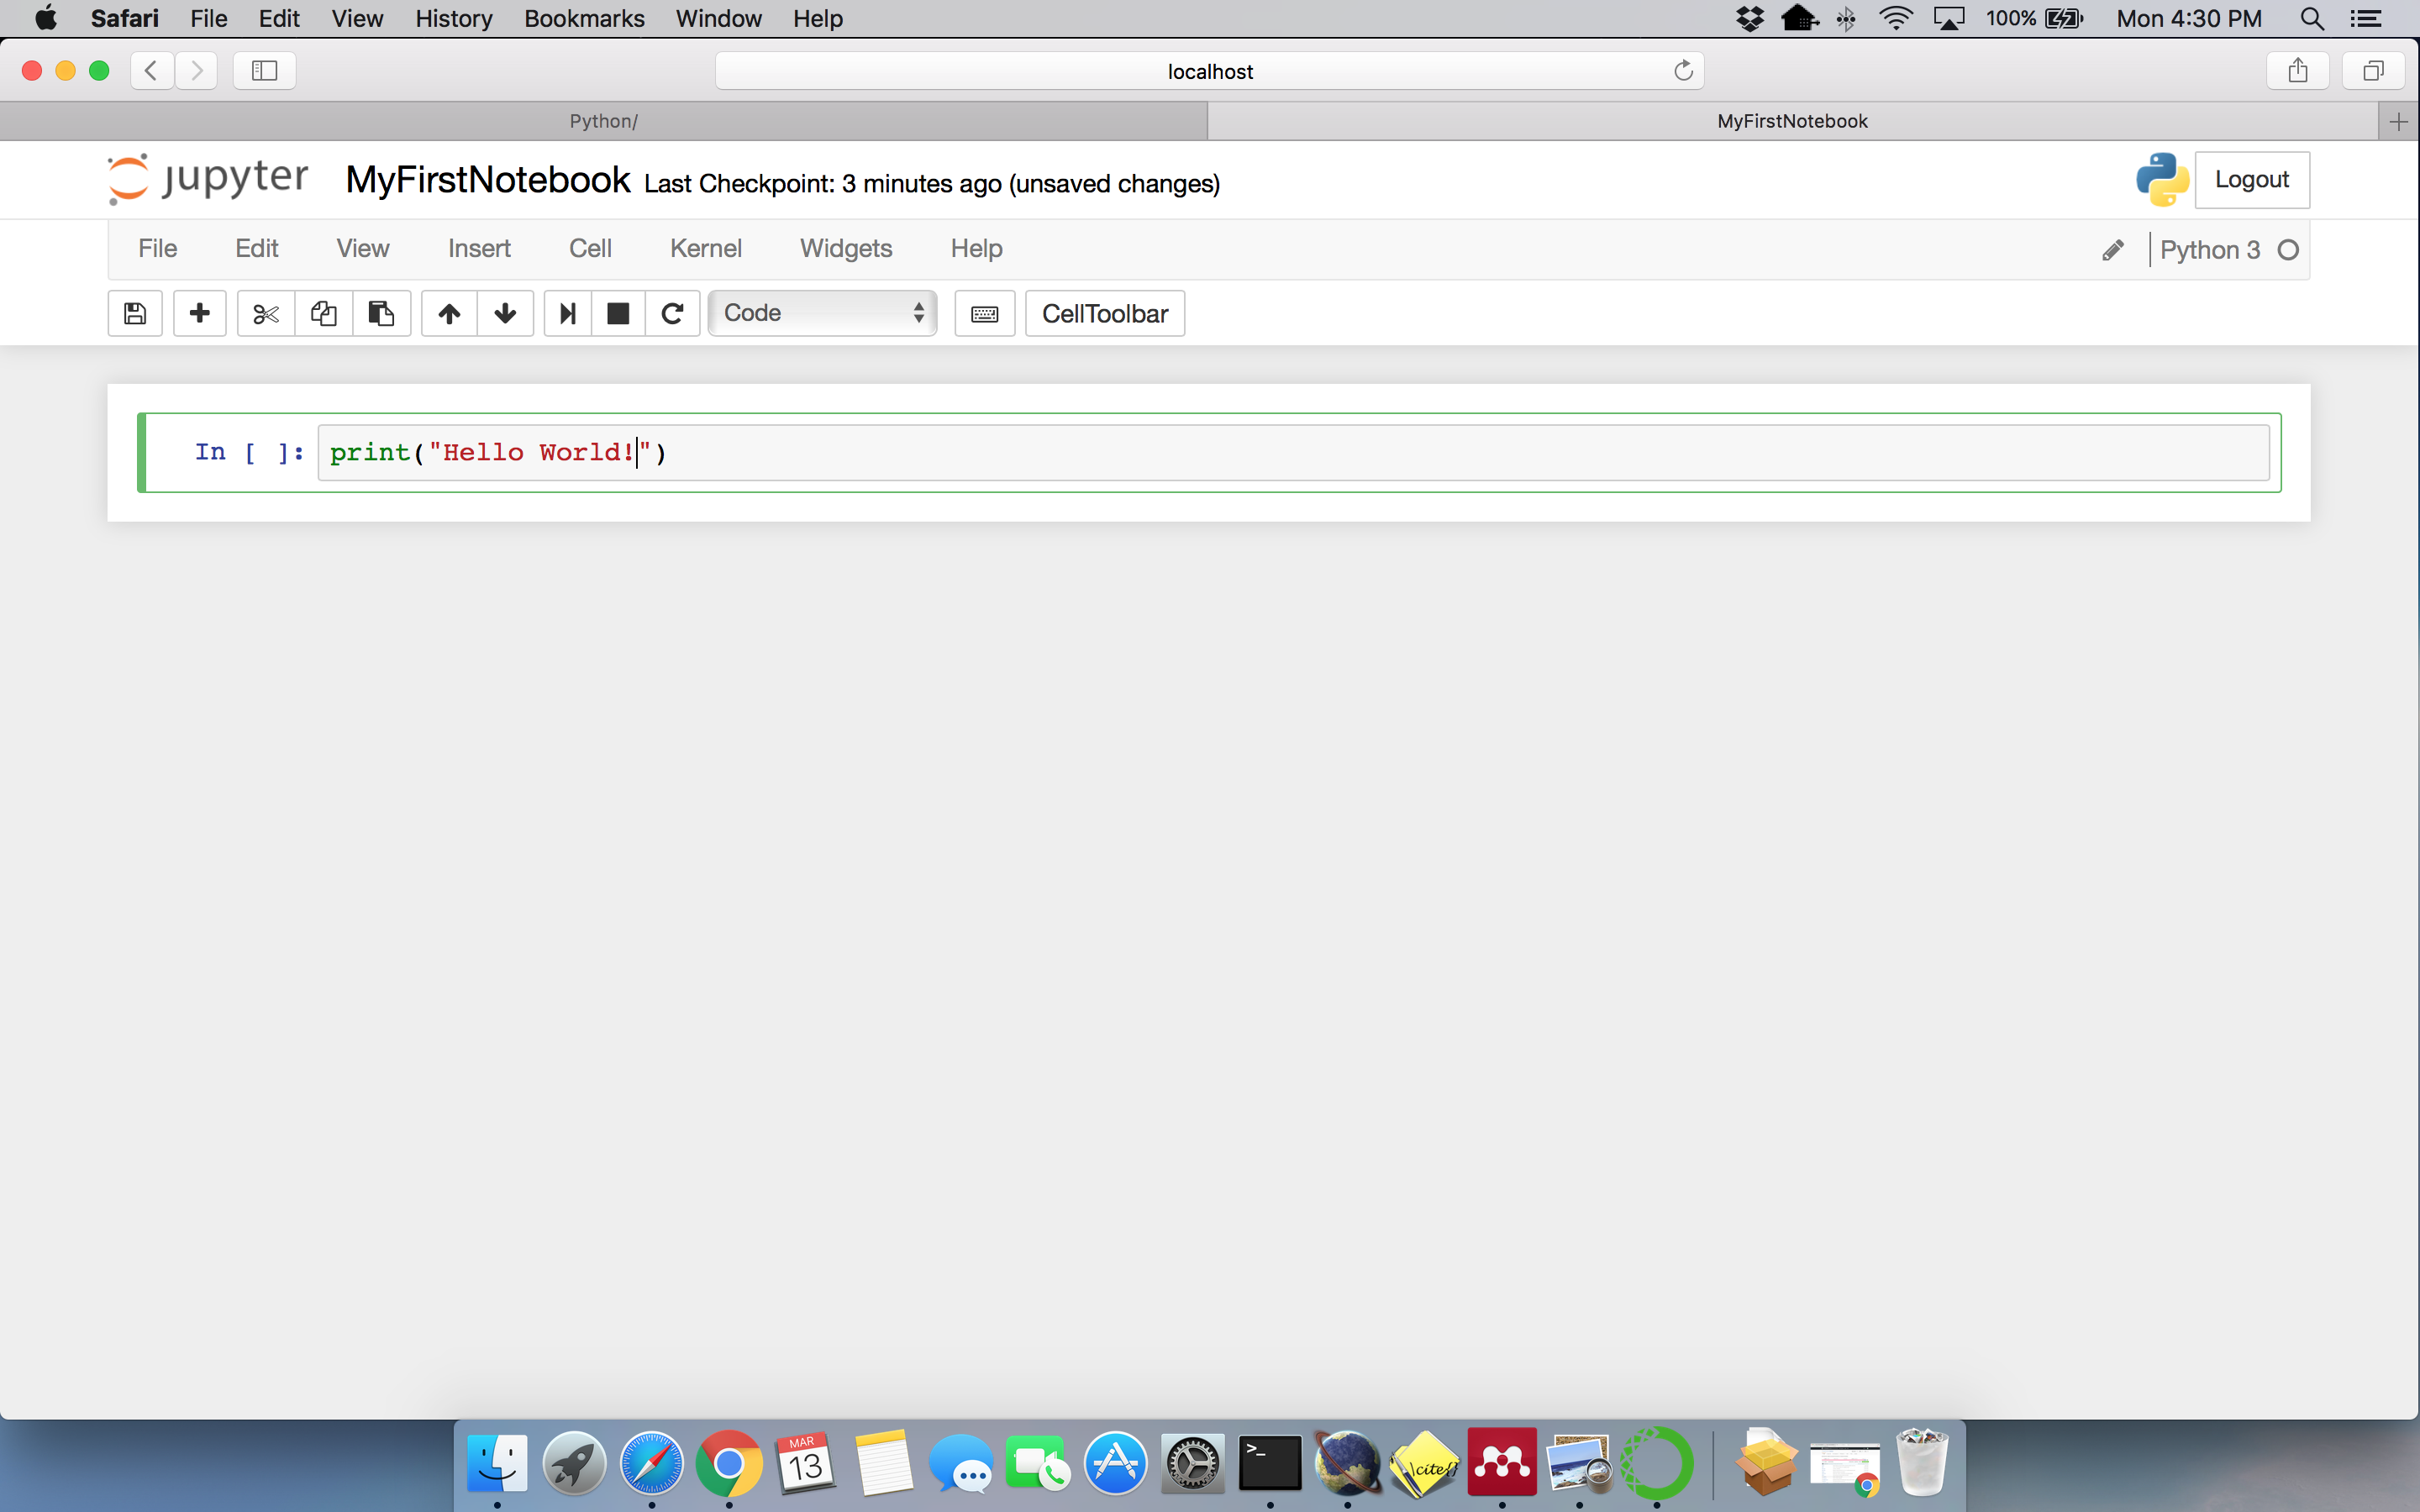
\includegraphics[scale=0.35]{Screenshot_23.png}}
\end{centering}

\paragraph{}
If you got something that looks like this picture, then congratulations! You just wrote your first Python program!
\paragraph{}
\begin{centering}
    \centerline{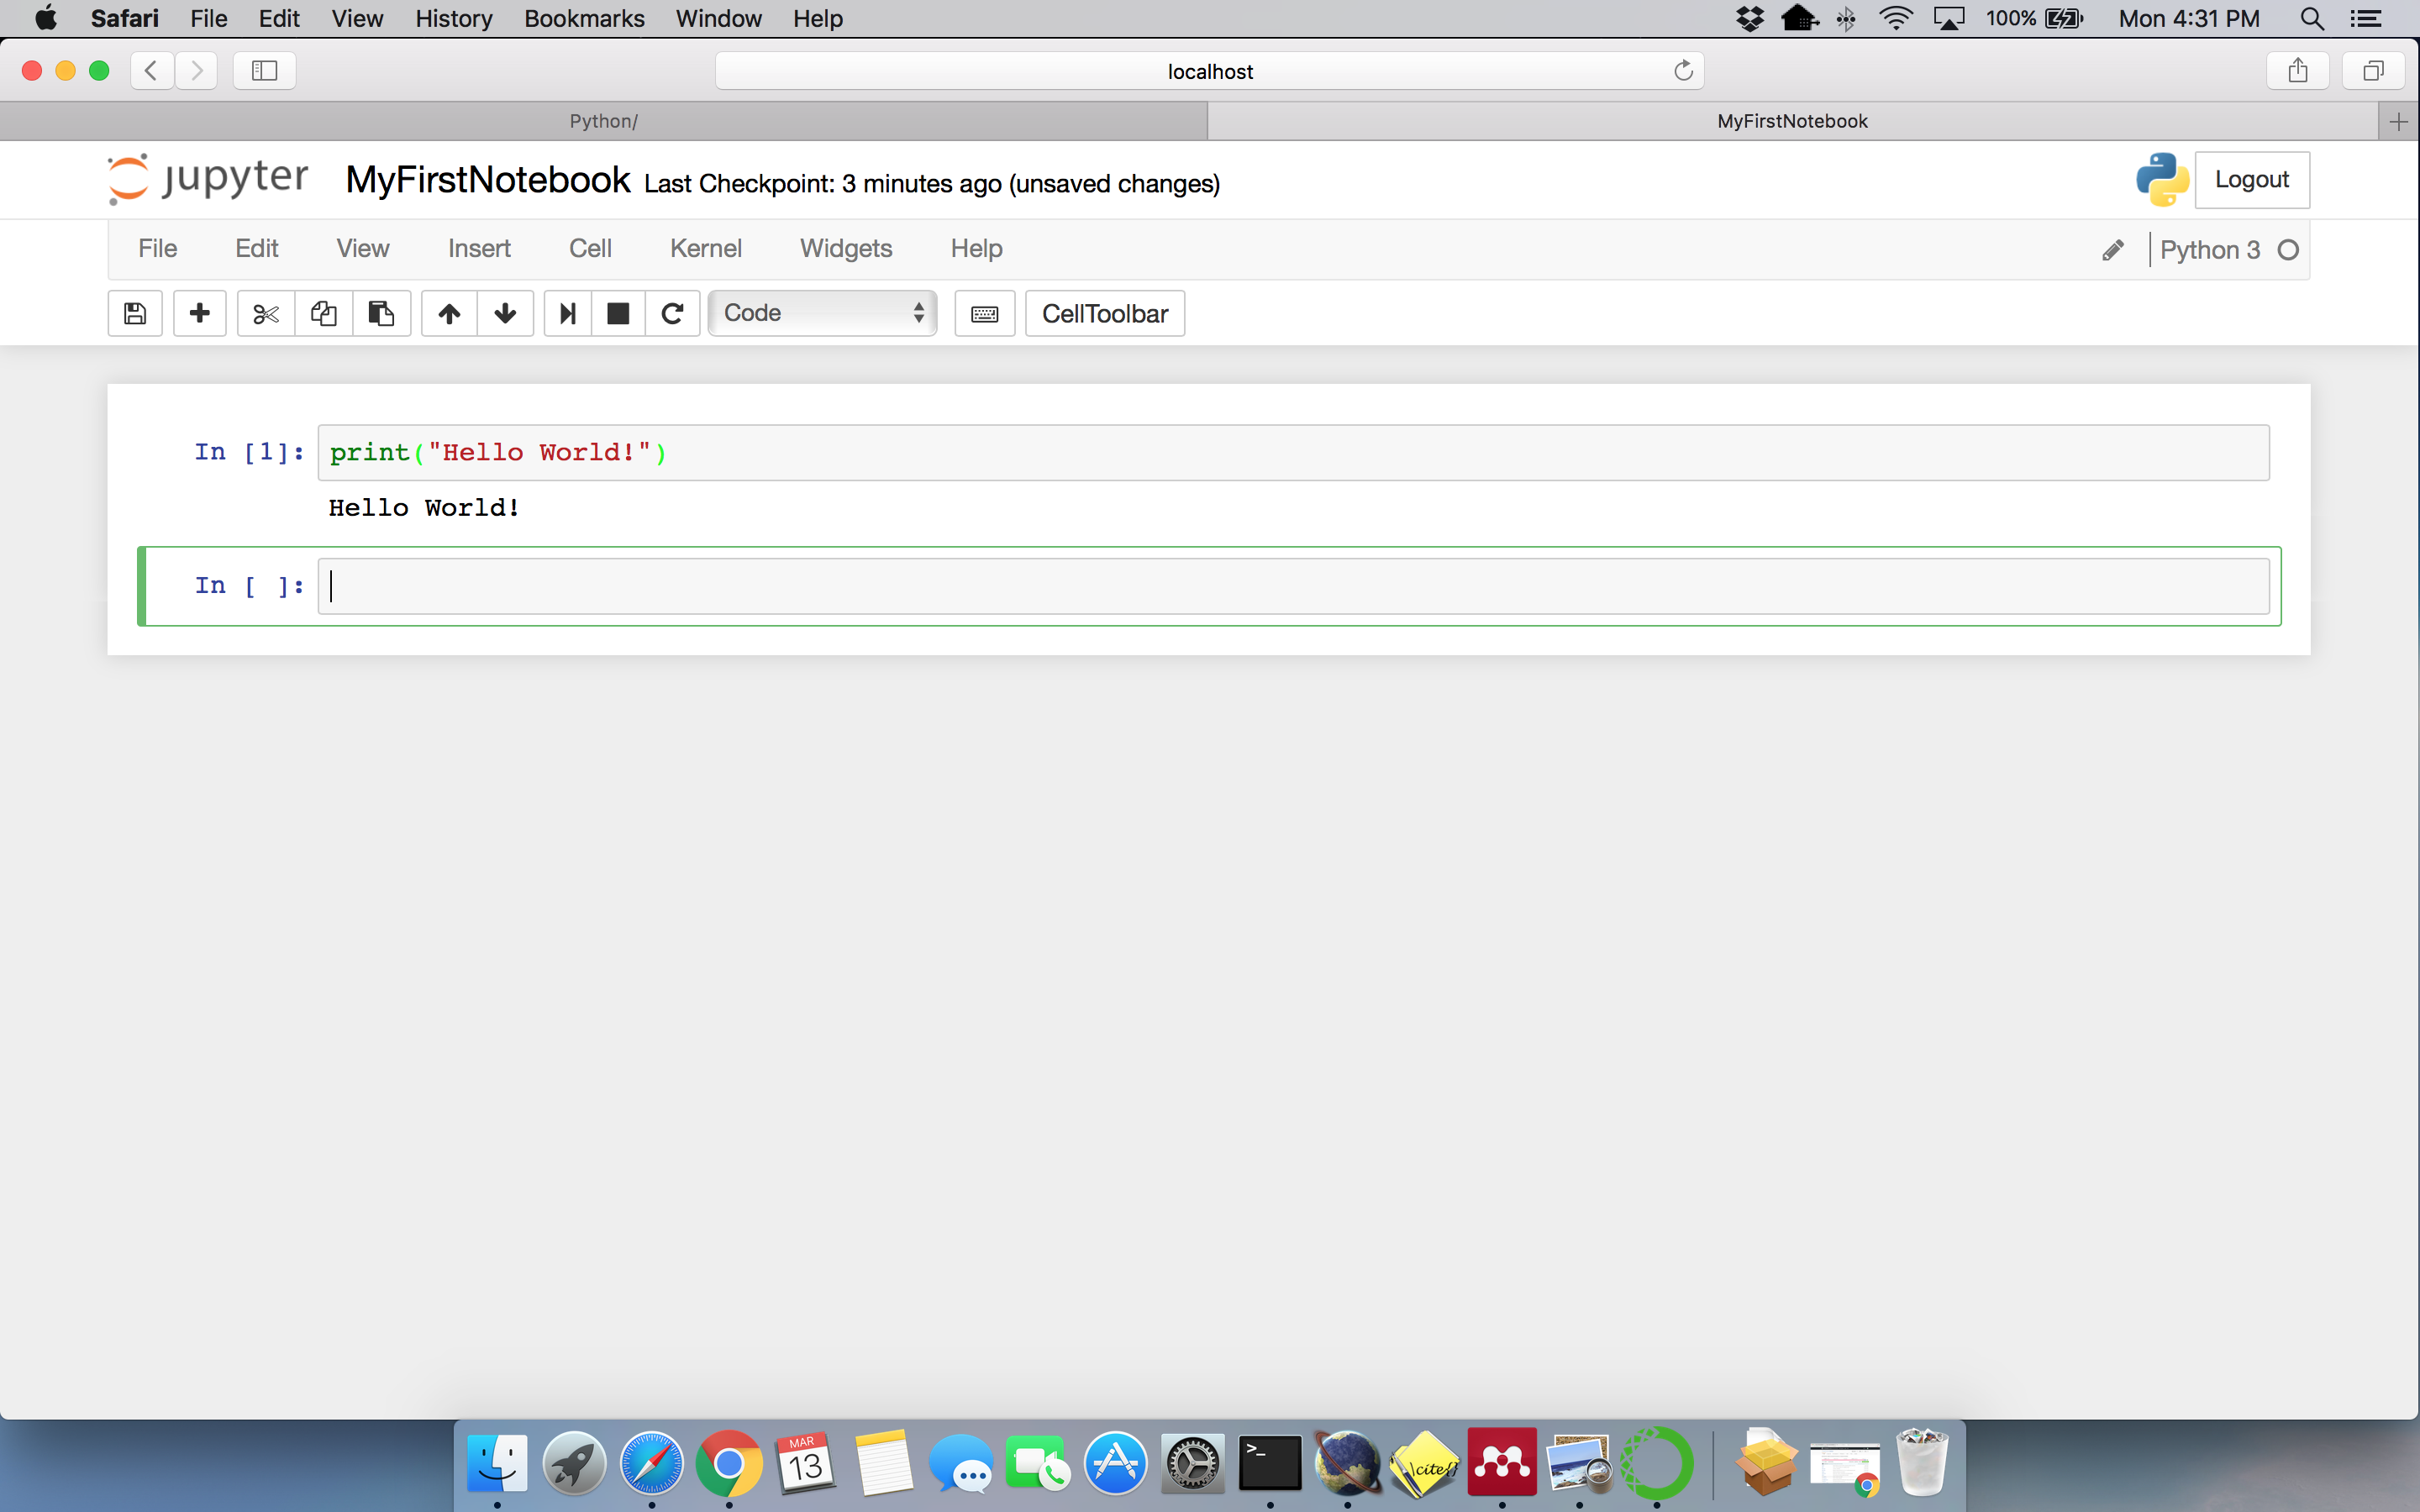
\includegraphics[scale=0.35]{Screenshot_24.png}}
\end{centering}

\paragraph{}
When you're finished, you can use File -- Save, and File -- Close and Halt to save your progress and exit out of the notebook.

\section*{Adding Files to Your Python Folder}
You may have received a number of Jupyter (or iPython) notebook files from the course instructors. You will need to be able to open these with the Jupyter program, which we just installed. To do this, you'll need to have those files downloaded somewhere on your computer. Then, with Jupyter open, go to the new folder (we simply named it "Python") that you created above. You should notice a button in the top right that says "Upload." Click this to open up a file explorer. Use this to add the notebooks we gave you to your Python folder (after selecting the file and confirming, you will have to click the blue upload button that appears next to the file name). This will allow you to open and read the notebooks that we provided.


\end{document}
